\section{Suche}
Dieses Kapitel beinhaltet die Beschreibung und Diskussion der vorgeschlagenen Suchresultate. Diese werden aufgeteilt
in einzelne Funktionsumfänge, da die Interpretation ansonsten zu komplex wird. Die Funktionsumfänge beschreiben die Suche
über einen einzelnen Stoss, über die Möglichkeit einer oder mehrerer Bandeninteraktionen, die Berücksichtigung verschiedener
Startgeschwindigkeiten und der vorausschauende Blick über mehrere Stösse.
Ein Suchresultat wird wiederum aufgrund vier verschiedener
Kriterien beurteilt. So spielt die Distanz des zurückzulegenden Weges, der Kollisionswinkel einzelner Kugeln, die Nähe
zum Loch einer einzulochenden Kugel und die benötigte Startgeschwindigkeit eine Rolle. Alle diese Kriterien werden für
jeden Vorschlag eines Stosses nach Segment aufgeschlüsselt. Ein Segment beschreibt den Weg von einer Kugel zur anderen
oder von einer Kugel zum Zielloch. Darin enthalten können mehrere Bandenkollisionen sein.

In einem ersten Teil wird sich nur der Suche über einen Stoss ohne Bandeninteraktion und ohne
vervielfältigter Startgeschwindigkeit gewidmet. Der zweite Teil beinhaltet zusätzlich verschiedene Startgeschwindigkeiten.
Im dritten Teil werden verschiedene Startgeschwindigkeiten wiederum ignoriert, aber dafür Bandeninteraktionen berücksichtigt.
Der vierte Teil beinhaltet den kompletten Funktionsumfang bis auf die Berücksichtigung verschiedener Startgeschwindigkeiten.

Um die Resultate der Suche zu bewerten, werden nachfolgend Situationen aufgestellt und die von der Suche
vorgeschlagenen Stösse auf Basis der Kriterien und berücksichtigten Funktionsumfänge untersucht.

\subsection{Die einfache Suche}\label{kap:suche:die_einfache_suche}
Die Situation zur einfachen Suche ist in Abbildung \ref{fig:search_situation_1} ersichtlich.
Der Spielball ist auf der linken Seite des Tisches und es liegen einige rote Kugeln auf dem Tisch verstreut.
Die Kugeln 1, 2 und 3 sind nahe bei den Löchern unten-links, oben-rechts resp. oben-zentral.
Kugel 4 ist in der Nähe des Spielballs, die Kugel 5 ist nahe dem Tischzentrum aufgestellt.

%
%State (for reproducing the results):
%WHITE1, WHITE, -564.147, 9.06096
%RED2, RED, -47.218, -100.06
%RED4, RED, 2.93182, 398.78
%RED5, RED, -865.047, -388.453
%RED6, RED, -629.728, 87.0048
%RED7, RED, 851.622, 398.78
%
\begin{figure}[h!]
    \begin{center}
        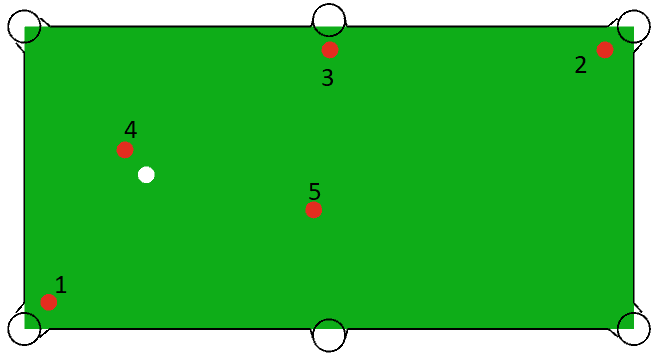
\includegraphics[width=0.4\linewidth]{../common/04_results/resources/simple_search/situation_diverse.PNG}
    \end{center}
    \caption{Situation 1: Einige verstreute Kugeln}
    \label{fig:search_situation_1}
\end{figure}

Nach Betrachten dieser Situation sind einige mögliche Stösse denkbar:
\begin{enumerate}
    \item Kugel 1 ins Loch unten-links.
    \item Kugel 2 ins Loch oben-rechts.
    \item Kugel 3 ins Loch oben-zentral.
    \item Kugel 4 ins Loch oben-links.
    \item Kugel 5 ins Loch unten-rechts.
    \item Kugel 5 ins Loch unten-zentral.
\end{enumerate}

In Abbildung \ref{fig:situation_1_solutions} sind die von der Suche gefundenen Stösse in aufsteigender Schwierigkeit abgebildet.
Mit den ersichtlichen weissen Linien auf jeder Abbildung ist der Pfad jeder Kugel, nicht nur des Spielballs, aufgezeichnet.
Diese voraussichtlichen Pfade werden nach der Suche mithilfe der Simulation des gefundenen Stosses eingezeichnet.

\begin{figure}[h!]
    \centering
    \begin{subfigure}[b]{0.3\textwidth}
        \centering
        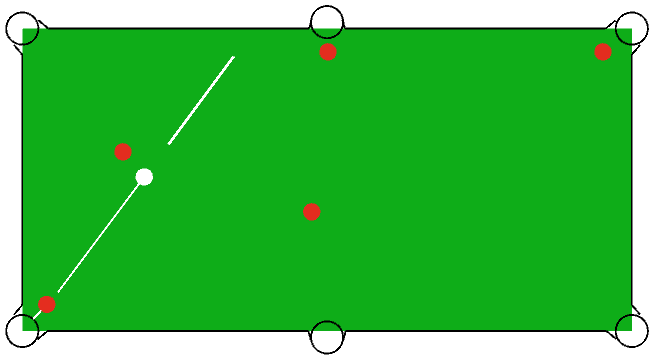
\includegraphics[width=1.0\linewidth]{../common/04_results/resources/simple_search/situation_diverse_solution_1.PNG}
        \caption{Stoss 1}
        \label{fig:situation_1_solution_1}
    \end{subfigure}
    \hfill
    \begin{subfigure}[b]{0.3\textwidth}
        \centering
        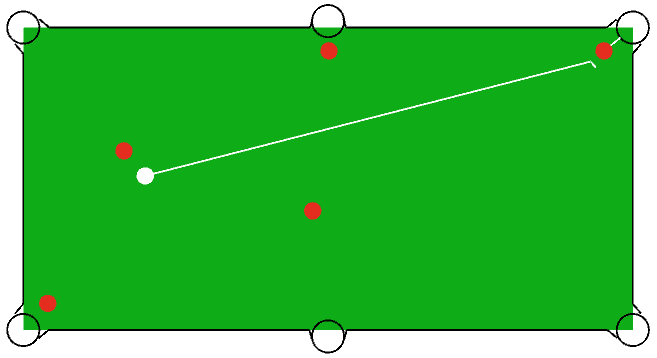
\includegraphics[width=1.0\linewidth]{../common/04_results/resources/simple_search/situation_diverse_solution_2.PNG}
        \caption{Stoss 2}
        \label{fig:situation_1_solution_2}
    \end{subfigure}
    \hfill
    \begin{subfigure}[b]{0.3\textwidth}
        \centering
        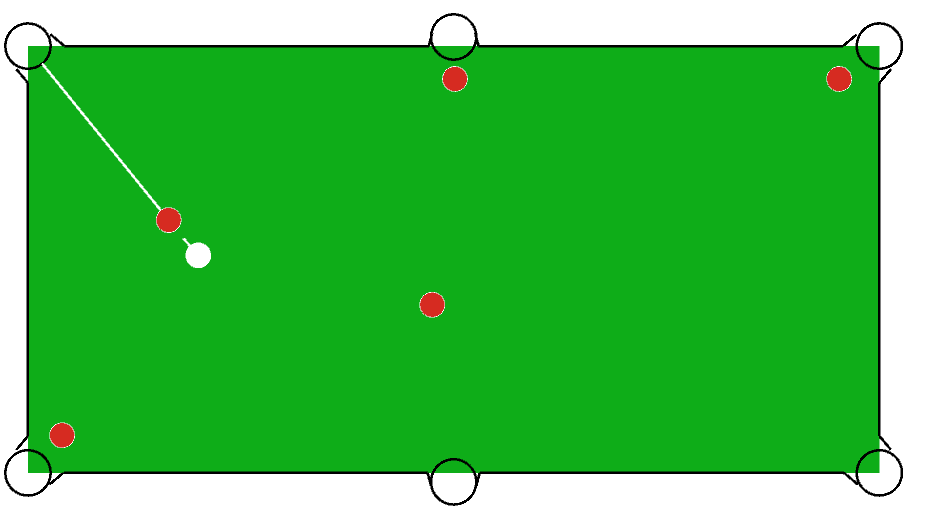
\includegraphics[width=1.0\linewidth]{../common/04_results/resources/simple_search/situation_diverse_solution_3.PNG}
        \caption{Stoss 3}
        \label{fig:situation_1_solution_3}
    \end{subfigure}
    \begin{subfigure}[b]{0.3\textwidth}
        \centering
        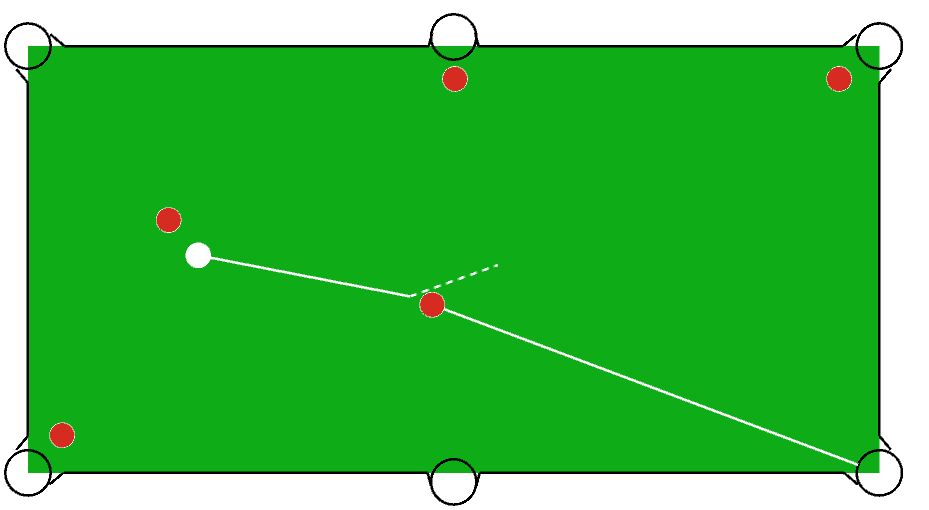
\includegraphics[width=1.0\linewidth]{../common/04_results/resources/simple_search/situation_diverse_solution_4.PNG}
        \caption{Stoss 4}
        \label{fig:situation_1_solution_4}
    \end{subfigure}
    \hfill
    \begin{subfigure}[b]{0.3\textwidth}
        \centering
        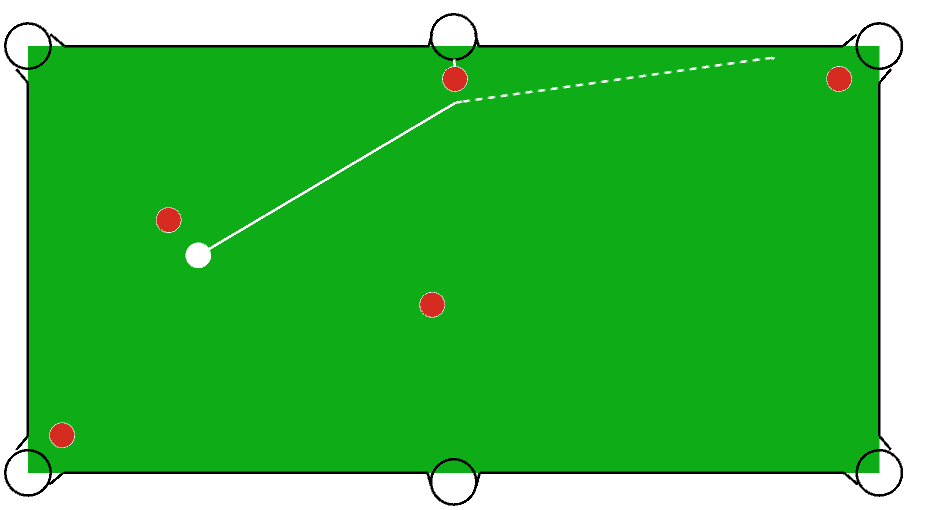
\includegraphics[width=1.0\linewidth]{../common/04_results/resources/simple_search/situation_diverse_solution_5.PNG}
        \caption{Stoss 5}
        \label{fig:situation_1_solution_5}
    \end{subfigure}
    \hfill
    \begin{subfigure}[b]{0.3\textwidth}
        \centering
        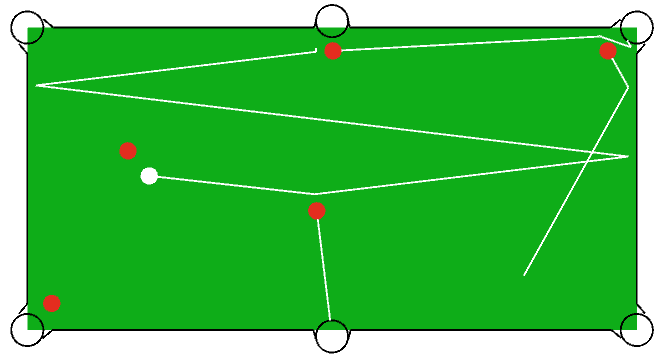
\includegraphics[width=1.0\linewidth]{../common/04_results/resources/simple_search/situation_diverse_solution_6.PNG}
        \caption{Stoss 6}
        \label{fig:situation_1_solution_6}
    \end{subfigure}
    \hfill
    \begin{subfigure}[b]{0.3\textwidth}
        \centering
        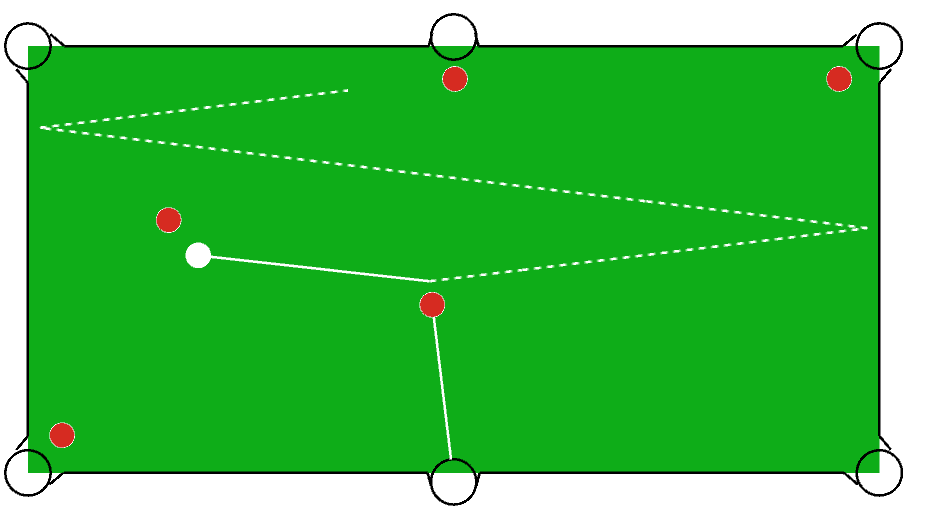
\includegraphics[width=1.0\linewidth]{../common/04_results/resources/simple_search/situation_diverse_solution_7.PNG}
        \caption{Stoss 7}
        \label{fig:situation_1_solution_7}
    \end{subfigure}
    \caption{Gefundene Stösse zu Situation 1 nach bewerteter Schwierigkeit aufsteigend}
    \label{fig:situation_1_solutions}
\end{figure}

Die zuvor beschriebenen denkbaren Stösse wurden tatsächlich gefunden.
Nach Tabelle \ref{tab:kosten_erster_vorschlag_ohne_bande_ohne_geschwindigkeit} wurde der Stoss 1 als der einfachste Stoss
bewertet, weil die gesamte zurückzulegende Distanz klein ist,
der Pfad der beteiligten Kugeln insgesamt sehr geradlinig ist und weil die Kugel 1 sehr nahe am Loch unten-links liegt.
Allgemein kann festgehalten werden, dass die Stösse in der Reihenfolge vorgeschlagen werden, wie es ihren totalen Suchkosten
entspricht.
Der zweiteinfachste Stoss 2 zeigt nach Tabelle \ref{tab:kosten_zweiter_vorschlag_ohne_bande_ohne_geschwindigkeit}
eine grössere Distanz, welche der Spielball zurücklegen muss und daher erfordert
der Stoss auch eine höhere Startgeschwindigkeit des Spielballs wodurch dieser als schwieriger eingestuft wird als Stoss 1.
Dafür ist die Kugel 2 sehr nahe am Loch oben-rechts, wodurch die Kugel nicht mit absoluter Genauigkeit getroffen werden
muss, damit diese den erwünschten Pfad nicht so weit verlässt, dass sie das Ziel verfehlt.

Im Stoss 3 ist die Gesamtdistanz nach Tabelle \ref{tab:kosten_dritter_vorschlag_ohne_bande_ohne_geschwindigkeit} klein,
allerdings ist die Distanz der Kugel 4 zum Spielball kleiner als die Distanz zum Loch.
Dadurch führt ein kleiner Fehler beim Treffen der Kugel zu einer grösseren Abweichung des Pfades.
In diesem Beispiel könnte dieser Fehler allerdings klein sein, da der Pfad geradlinig ist und der Spielball die Kugel
nicht in einem Winkel treffen muss.

Stoss 2 wurde besser als Stoss 3 bewertet, weil bei Stoss 2 die Kugel näher am Loch liegt als bei Stoss 3. Die anderen
Bewertungskriterien Distanz und Winkel des Segments \glqq Weiss - Rot\grqq{} sind bei Stoss 3 besser als bei Stoss 2.
Ob diese Rangfolge objektiv korrekt ist, ist schwierig zu beurteilen.

Der Stoss 5 wird nach Tabelle \ref{tab:kosten_fuenfter_vorschlag_ohne_bande_ohne_geschwindigkeit} als schwieriger bewertet, weil der Winkel, in dem der Spielball die Kugel 3 treffen muss, ca. 45$^{\circ}$ ist.
Im Gegensatz dazu ist die Distanz der Kugel zum Loch sehr klein und die Gesamtdistanz ist relativ klein, was diesen Stoss
wiederum einfacher macht. Trotzdem hat in diesem Fall der Winkel die Bewertung so stark reduziert, dass Stoss 4 nach
Tabelle \ref{tab:kosten_vierter_vorschlag_ohne_bande_ohne_geschwindigkeit} trotz allem als einfacher eingestuft wird.

Der Stoss 6 versenkt die Kugel 2 indirekt über die Kugel 5. Dieser Stoss wird nach
Tabelle \ref{tab:kosten_sechster_vorschlag_ohne_bande_ohne_geschwindigkeit} dennoch einfacher bewertet als der
nachfolgende Stoss 7, der keine Indirektion beinhaltet, da der Auftrittswinkel nicht so gross ist und die weisse Kugel
nicht so stark angespielt werden muss.

Stoss 7 zeigt die Idee, Kugel 5 ins Loch unten-zentral zu spielen.
Dazu muss diese nach Tabelle \ref{tab:kosten_siebter_vorschlag_ohne_bande_ohne_geschwindigkeit} in einem sehr grossen
Winkel angespielt werden, was die Treffgenauigkeit reduziert und eine erhöhte Startgeschwindigkeit des Spielballs erfordert.

Aus den obigen Resultaten ist ersichtlich, dass die Suche diejenigen Stösse vorschlägt, welche nach Studium des Spielstandes
möglich erscheinen. Zudem berücksichtigt die Bewertung der Schwierigkeit eines Stosses die gesamte Distanz, die Winkel, die Nähe
der einzulochenden Kugel zum Loch und die erforderliche Startgeschwindigkeit.

%[mapToSolution] COST START
%[mapToSolution] cost-search - distance: 0 angle: 0 indirection: 0 sum: 0 cost: 0 previous cost: 0 total cost: 0
%[mapToSolution] cost-search - distance: 0.00284364 angle: 3.93338e-06 indirection: 0 sum: 0.00284757 cost: 284 previous cost: 0 total cost: 284
%[mapToSolution] cost-search - distance: 0.000128041 angle: 7.48246e-05 indirection: 0.5 sum: 0.500203 cost: 50020 previous cost: 284 total cost: 50304
%[mapToSolution] cost-simulation - cost: 21902 previous cost: 50304 total cost: 72206
%[mapToSolution] end cost: 72206
%[mapToSolution] COST END
\begin{table}[h!]
    \rowcolors{1}{\seccolor!10}{\seccolor!10} % Rows with 10% of secondary color
    \begin{tabular}{llrrrr}
        \rowcolor{\seccolor!50}
        Stoss & Segment & Distanzkosten & Winkelkosten & Indirektionskosten & Total (Ganzzahl)\\\bfhmidline
        1          & Weiss - Rot & 0.00012804  & 0.0000748246  & 0.5 & 50020 \\
        1          & Rot - Loch  & 0.00284364  & 0.0000039334  & 0   & 284 \\
        \textbf{1} & \multicolumn{4}{l}{\textbf{Suchkostentotal}}    & \textbf{50304}\\
        1          & Simulation & \multicolumn{4}{r}{21902}\\\bfhmidline
        \multicolumn{5}{l}{\textbf{Gesamttotal}}                     & \textbf{72206}\\
    \end{tabular}
    \caption{Kosten des ersten Vorschlags über einen einfachen Stoss ohne Bandeninteraktion und vervielfältigter Geschwindigkeit.}
    \label{tab:kosten_erster_vorschlag_ohne_bande_ohne_geschwindigkeit}
\end{table}

%[mapToSolution] COST START
%[mapToSolution] cost-search - distance: 0 angle: 0 indirection: 0 sum: 0 cost: 0 previous cost: 0 total cost: 0
%[mapToSolution] cost-search - distance: 0.0029786 angle: 7.36014e-05 indirection: 0 sum: 0.0030522 cost: 305 previous cost: 0 total cost: 305
%[mapToSolution] cost-search - distance: 0.00135804 angle: 0.0237772 indirection: 0.5 sum: 0.525135 cost: 52513 previous cost: 305 total cost: 52818
%[mapToSolution] cost-simulation - cost: 23547 previous cost: 52818 total cost: 76365
%[mapToSolution] end cost: 76365
%[mapToSolution] COST END
\begin{table}[h!]
    \rowcolors{1}{\seccolor!10}{\seccolor!10} % Rows with 10% of secondary color
    \begin{tabular}{llrrrr}
        \rowcolor{\seccolor!50}
        Stoss & Segment & Distanzkosten & Winkelkosten & Indirektionskosten & Total (Ganzzahl)\\\bfhmidline
        1          & Weiss - Rot & 0.001358    & 0.0237772     & 0.5 & 52513 \\
        1          & Rot - Loch  & 0.0029786   & 0.0000736     & 0   & 305 \\
        \textbf{1} & \multicolumn{4}{l}{\textbf{Suchkostentotal}}    & \textbf{52818}\\
        1          & Simulation & \multicolumn{4}{r}{23547}\\\bfhmidline
        \multicolumn{5}{l}{\textbf{Gesamttotal}}                     & \textbf{76365}\\
    \end{tabular}
    \caption{Kosten des zweiten Vorschlags über einen einfachen Stoss ohne Bandeninteraktion und vervielfältigter Geschwindigkeit.}
    \label{tab:kosten_zweiter_vorschlag_ohne_bande_ohne_geschwindigkeit}
\end{table}

%[mapToSolution] COST START
%[mapToSolution] cost-search - distance: 0 angle: 0 indirection: 0 sum: 0 cost: 0 previous cost: 0 total cost: 0
%[mapToSolution] cost-search - distance: 0.0552051 angle: 9.28795e-05 indirection: 0 sum: 0.055298 cost: 5529 previous cost: 0 total cost: 5529
%[mapToSolution] cost-search - distance: 3.0656e-05 angle: 2.01923e-06 indirection: 0.5 sum: 0.500033 cost: 50003 previous cost: 5529 total cost: 55532
%[mapToSolution] cost-simulation - cost: 24388 previous cost: 55532 total cost: 79920
%[mapToSolution] end cost: 79920
%[mapToSolution] COST END
\begin{table}[h!]
    \rowcolors{1}{\seccolor!10}{\seccolor!10} % Rows with 10% of secondary color
    \begin{tabular}{llrrrr}
        \rowcolor{\seccolor!50}
        Stoss & Segment & Distanzkosten & Winkelkosten & Indirektionskosten & Total (Ganzzahl)\\\bfhmidline
        1          & Weiss - Rot & 0.0000307    & 0.0000020193  & 0.5 & 50003 \\
        1          & Rot - Loch  & 0.0552051    & 0.0000928795  & 0   & 5529 \\
        \textbf{1} & \multicolumn{4}{l}{\textbf{Suchkostentotal}}     & \textbf{55532}\\
        1          & Simulation & \multicolumn{4}{r}{24388}\\\bfhmidline
        \multicolumn{5}{l}{\textbf{Gesamttotal}}                      & \textbf{79920}\\
    \end{tabular}
    \caption{Kosten des dritten Vorschlags über einen einfachen Stoss ohne Bandeninteraktion und vervielfältigter Geschwindigkeit.}
    \label{tab:kosten_dritter_vorschlag_ohne_bande_ohne_geschwindigkeit}
\end{table}

%[mapToSolution] COST START
%[mapToSolution] cost-search - distance: 0 angle: 0 indirection: 0 sum: 0 cost: 0 previous cost: 0 total cost: 0
%[mapToSolution] cost-search - distance: 0.251514 angle: 0.0224747 indirection: 0 sum: 0.273988 cost: 27398 previous cost: 0 total cost: 27398
%[mapToSolution] cost-search - distance: 0.0129086 angle: 0.000592332 indirection: 0.5 sum: 0.513501 cost: 51350 previous cost: 27398 total cost: 78748
%[mapToSolution] cost-simulation - cost: 35872 previous cost: 78748 total cost: 114620
%[mapToSolution] end cost: 114620
%[mapToSolution] COST END
\begin{table}[h!]
    \rowcolors{1}{\seccolor!10}{\seccolor!10} % Rows with 10% of secondary color
    \begin{tabular}{llrrrr}
        \rowcolor{\seccolor!50}
        Stoss & Segment & Distanzkosten & Winkelkosten & Indirektionskosten & Total (Ganzzahl)\\\bfhmidline
        1          & Weiss - Rot & 0.012909     & 0.0005923     & 0.5 & 51350 \\
        1          & Rot - Loch  & 0.251514     & 0.0224747     & 0   & 27398 \\
        \textbf{1} & \multicolumn{4}{l}{\textbf{Suchkostentotal}}     & \textbf{78748}\\
        1          & Simulation & \multicolumn{4}{r}{35872}\\\bfhmidline
        \multicolumn{5}{l}{\textbf{Gesamttotal}}                      & \textbf{114620}\\
    \end{tabular}
    \caption{Kosten des vierten Vorschlags über einen einfachen Stoss ohne Bandeninteraktion und vervielfältigter Geschwindigkeit.}
    \label{tab:kosten_vierter_vorschlag_ohne_bande_ohne_geschwindigkeit}
\end{table}

%[mapToSolution] COST START
%[mapToSolution] cost-search - distance: 0 angle: 0 indirection: 0 sum: 0 cost: 0 previous cost: 0 total cost: 0
%[mapToSolution] cost-search - distance: 0.00194371 angle: 7.48391e-07 indirection: 0 sum: 0.00194446 cost: 194 previous cost: 0 total cost: 194
%[mapToSolution] cost-search - distance: 0.000191993 angle: 0.525736 indirection: 0.5 sum: 1.02593 cost: 102592 previous cost: 194 total cost: 102786
%[mapToSolution] cost-simulation - cost: 45576 previous cost: 102786 total cost: 148362
%[mapToSolution] end cost: 148362
%[mapToSolution] COST END
\begin{table}[h!]
    \rowcolors{1}{\seccolor!10}{\seccolor!10} % Rows with 10% of secondary color
    \begin{tabular}{llrrrr}
        \rowcolor{\seccolor!50}
        Stoss & Segment & Distanzkosten & Winkelkosten & Indirektionskosten & Total (Ganzzahl)\\\bfhmidline
        1          & Weiss - Rot & 0.000192      & 0.525736      & 0.5 & 102592 \\
        1          & Rot - Loch  & 0.001944      & 0.0000007484  & 0   & 194 \\
        \textbf{1} & \multicolumn{4}{l}{\textbf{Suchkostentotal}}      & \textbf{102786}\\
        1          & Simulation & \multicolumn{4}{r}{45576}\\\bfhmidline
        \multicolumn{5}{l}{\textbf{Gesamttotal}}                       & \textbf{148362}\\
    \end{tabular}
    \caption{Kosten des fünften Vorschlags über einen einfachen Stoss ohne Bandeninteraktion und vervielfältigter Geschwindigkeit.}
    \label{tab:kosten_fuenfter_vorschlag_ohne_bande_ohne_geschwindigkeit}
\end{table}

%[mapToSolution] COST START
%[mapToSolution] cost-search - distance: 0 angle: 0 indirection: 0 sum: 0 cost: 0 previous cost: 0 total cost: 0
%[mapToSolution] cost-search - distance: 0.0029786 angle: 7.36014e-05 indirection: 0 sum: 0.0030522 cost: 305 previous cost: 0 total cost: 305
%[mapToSolution] cost-search - distance: 0.215404 angle: 0.000932547 indirection: 0.5 sum: 0.716337 cost: 71633 previous cost: 305 total cost: 71938
%[mapToSolution] cost-search - distance: 0.0116657 angle: 0.197609 indirection: 0.5 sum: 0.709275 cost: 70927 previous cost: 71938 total cost: 142865
%[mapToSolution] cost-simulation - cost: 68868 previous cost: 142865 total cost: 211733
%[mapToSolution] end cost: 211733
%[mapToSolution] COST END
\begin{table}[h!]
    \rowcolors{1}{\seccolor!10}{\seccolor!10} % Rows with 10% of secondary color
    \begin{tabular}{llrrrr}
        \rowcolor{\seccolor!50}
        Stoss & Segment & Distanzkosten & Winkelkosten & Indirektionskosten & Total (Ganzzahl)\\\bfhmidline
        1          & Weiss - Rot & 0.011666       & 0.197609      & 0.5 & 70927 \\
        1          & Rot - Rot   & 0.215404       & 0.0009326     & 0.5 & 71633 \\
        1          & Rot - Loch  & 0.002979       & 0.0000736     & 0   & 305 \\
        \textbf{1} & \multicolumn{4}{l}{\textbf{Suchkostentotal}}       & \textbf{142865}\\
        1          & Simulation & \multicolumn{4}{r}{68868}\\\bfhmidline
        \multicolumn{5}{l}{\textbf{Gesamttotal}}                        & \textbf{211733}\\
    \end{tabular}
    \caption{Kosten des sechsten Vorschlags über einen einfachen Stoss ohne Bandeninteraktion und vervielfältigter Geschwindigkeit.}
    \label{tab:kosten_sechster_vorschlag_ohne_bande_ohne_geschwindigkeit}
\end{table}

%[mapToSolution] COST START
%[mapToSolution] cost-search - distance: 0 angle: 0 indirection: 0 sum: 0 cost: 0 previous cost: 0 total cost: 0
%[mapToSolution] cost-search - distance: 0.0351119 angle: 0.000154641 indirection: 0 sum: 0.0352666 cost: 3526 previous cost: 0 total cost: 3526
%[mapToSolution] cost-search - distance: 0.00209408 angle: 0.866141 indirection: 0.5 sum: 1.36824 cost: 136823 previous cost: 3526 total cost: 140349
%[mapToSolution] cost-simulation - cost: 82303 previous cost: 140349 total cost: 222652
%[mapToSolution] end cost: 222652
%[mapToSolution] COST END
\begin{table}[h!]
    \rowcolors{1}{\seccolor!10}{\seccolor!10} % Rows with 10% of secondary color
    \begin{tabular}{llrrrr}
        \rowcolor{\seccolor!50}
        Stoss & Segment & Distanzkosten & Winkelkosten & Indirektionskosten & Total (Ganzzahl)\\\bfhmidline
        1          & Weiss - Rot & 0.00209408     & 0.866141      & 0.5 & 136823 \\
        1          & Rot - Loch  & 0.0351119      & 0.000155      & 0   & 3526 \\
        \textbf{1} & \multicolumn{4}{l}{\textbf{Suchkostentotal}}       & \textbf{140349}\\
        1          & Simulation & \multicolumn{4}{r}{82303}\\\bfhmidline
        \multicolumn{5}{l}{\textbf{Gesamttotal}}                        & \textbf{222652}\\
    \end{tabular}
    \caption{Kosten des siebten Vorschlags über einen einfachen Stoss ohne Bandeninteraktion und vervielfältigter Geschwindigkeit.}
    \label{tab:kosten_siebter_vorschlag_ohne_bande_ohne_geschwindigkeit}
\end{table}

\clearpage
\subsection{Die einfache Suche - mit vervielfältigter Startgeschwindigkeit}
Es wird wiederum die Situation wie in Kapitel \ref{kap:suche:die_einfache_suche} betrachtet. Diesmal wird aber die Vervielfältigung der Startgeschwindigkeiten
zugelassen, insgesamt werden jeweils drei verschieden starke Stargeschwindigkeiten berücksichtigt.
Als Resultat wird in etwa dieselbe Abfolge der Suchresultate wie in Kapitel \ref{kap:suche:die_einfache_suche} erwartet, es kann aber durchaus
sein, dass gewisse Stösse mit geringer Distanz und kleinem Winkel durch die hohe Startgeschwindigkeit schlechter bewertet werden
als solche mit grösserer Distanz und grösserem Winkel.

In Abbildung \ref{fig:situation_1_solutions_startgeschwindigkeit} sind die von der Suche gefundenen Stösse in aufsteigender Schwierigkeit abgebildet.
Insgesamt wurden 21 Lösungen gefunden, davon werden nur die zehn besten diskutiert.

\begin{figure}[h!]
    \centering
    \begin{subfigure}[b]{0.3\textwidth}
        \centering
        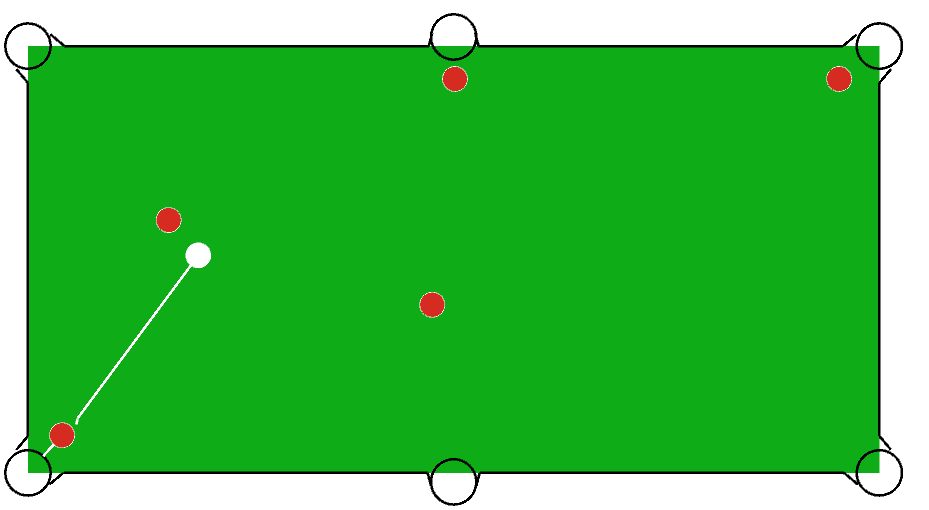
\includegraphics[width=1.0\linewidth]{../common/04_results/resources/simple_search/situation_diverse_solution_velocity_1.PNG}
        \caption{Stoss 1}
        \label{fig:situation_velocity_1_solution_1}
    \end{subfigure}
    \hfill
    \begin{subfigure}[b]{0.3\textwidth}
        \centering
        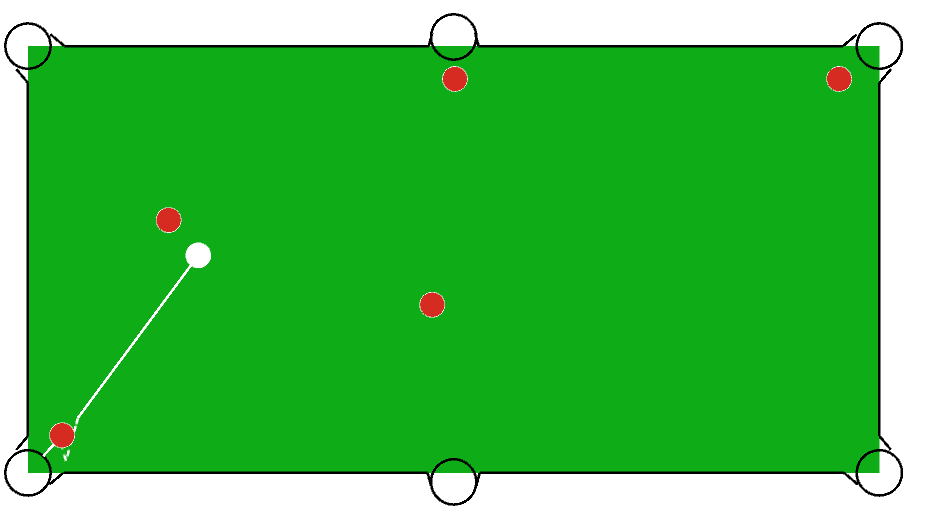
\includegraphics[width=1.0\linewidth]{../common/04_results/resources/simple_search/situation_diverse_solution_velocity_2.PNG}
        \caption{Stoss 2}
        \label{fig:situation_velocity_1_solution_2}
    \end{subfigure}
    \hfill
    \begin{subfigure}[b]{0.3\textwidth}
        \centering
        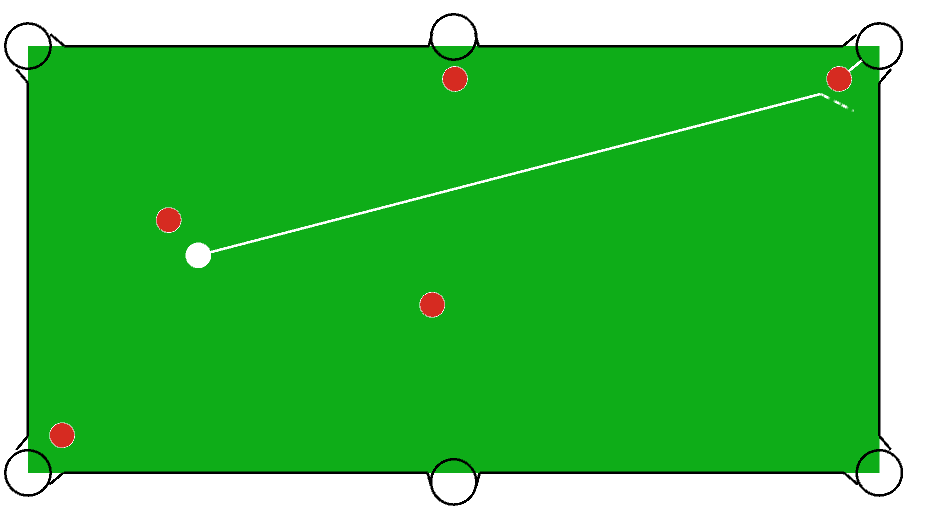
\includegraphics[width=1.0\linewidth]{../common/04_results/resources/simple_search/situation_diverse_solution_velocity_3.PNG}
        \caption{Stoss 3}
        \label{fig:situation_velocity_1_solution_3}
    \end{subfigure}
    \hfill
    \begin{subfigure}[b]{0.3\textwidth}
        \centering
        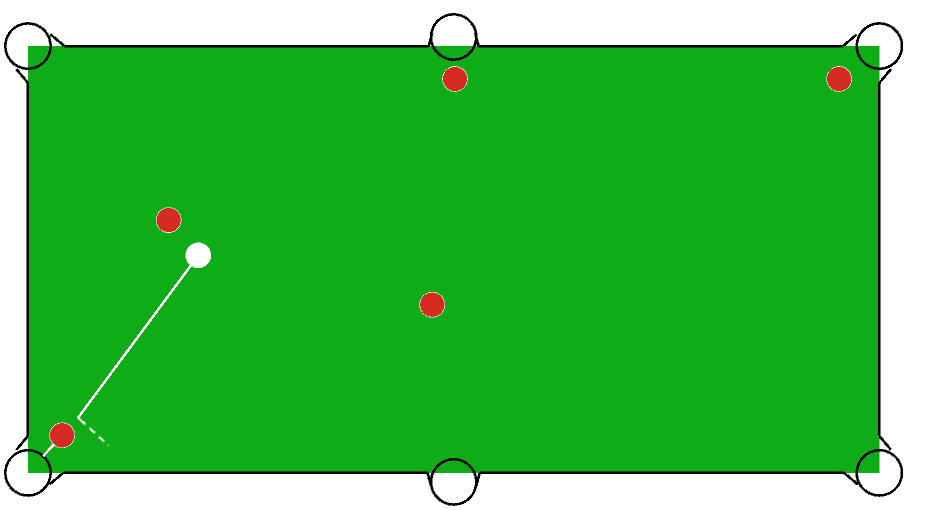
\includegraphics[width=1.0\linewidth]{../common/04_results/resources/simple_search/situation_diverse_solution_velocity_4.PNG}
        \caption{Stoss 4}
        \label{fig:situation_velocity_1_solution_4}
    \end{subfigure}
    \hfill
    \begin{subfigure}[b]{0.3\textwidth}
        \centering
        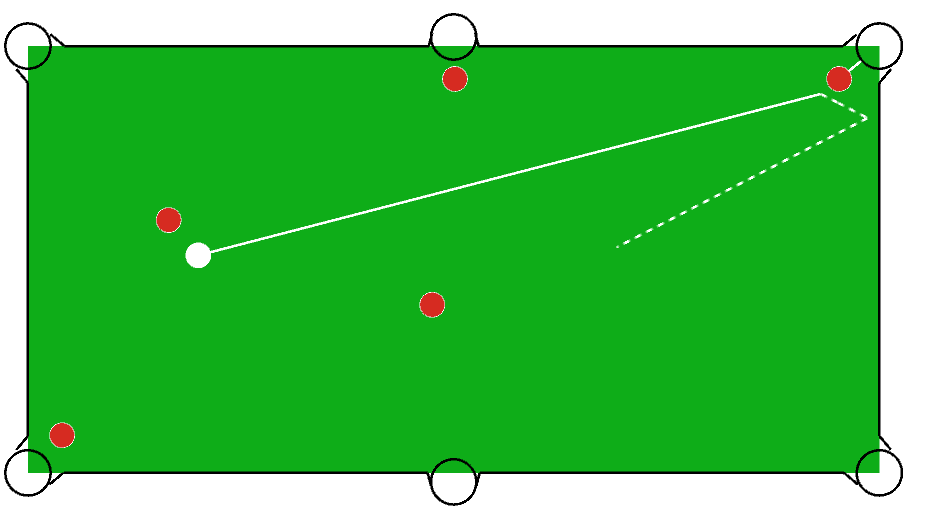
\includegraphics[width=1.0\linewidth]{../common/04_results/resources/simple_search/situation_diverse_solution_velocity_5.PNG}
        \caption{Stoss 5}
        \label{fig:situation_velocity_1_solution_5}
    \end{subfigure}
    \hfill
    \begin{subfigure}[b]{0.3\textwidth}
        \centering
        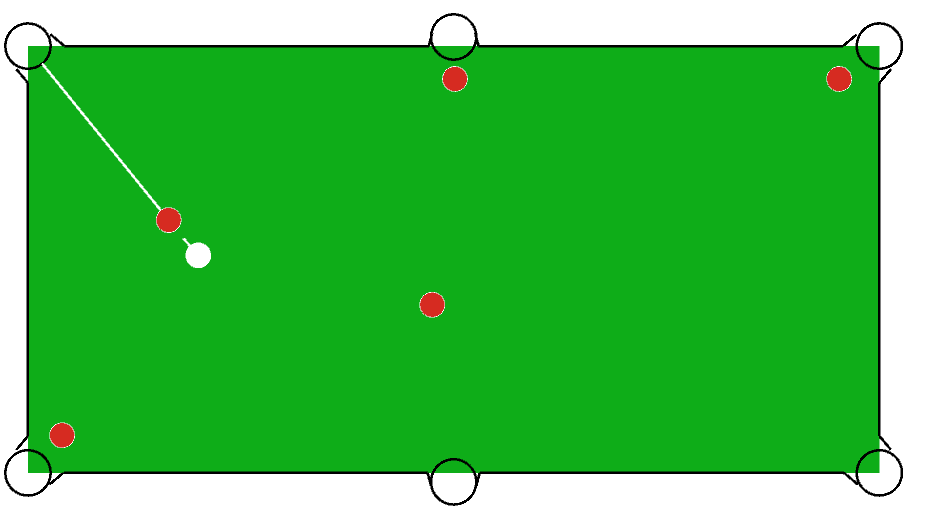
\includegraphics[width=1.0\linewidth]{../common/04_results/resources/simple_search/situation_diverse_solution_velocity_6.PNG}
        \caption{Stoss 6}
        \label{fig:situation_velocity_1_solution_6}
    \end{subfigure}
    \hfill
    \begin{subfigure}[b]{0.3\textwidth}
        \centering
        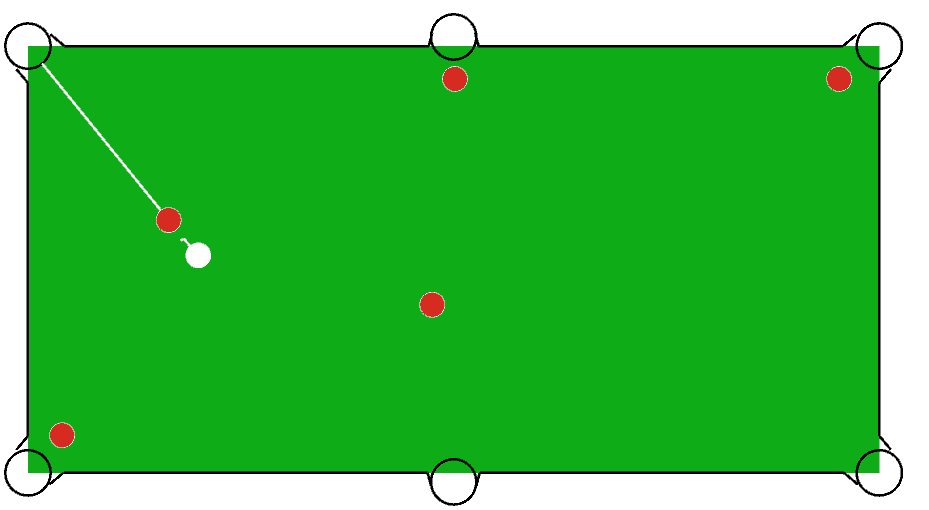
\includegraphics[width=1.0\linewidth]{../common/04_results/resources/simple_search/situation_diverse_solution_velocity_7.PNG}
        \caption{Stoss 7}
        \label{fig:situation_velocity_1_solution_7}
    \end{subfigure}
    \hfill
    \begin{subfigure}[b]{0.3\textwidth}
        \centering
        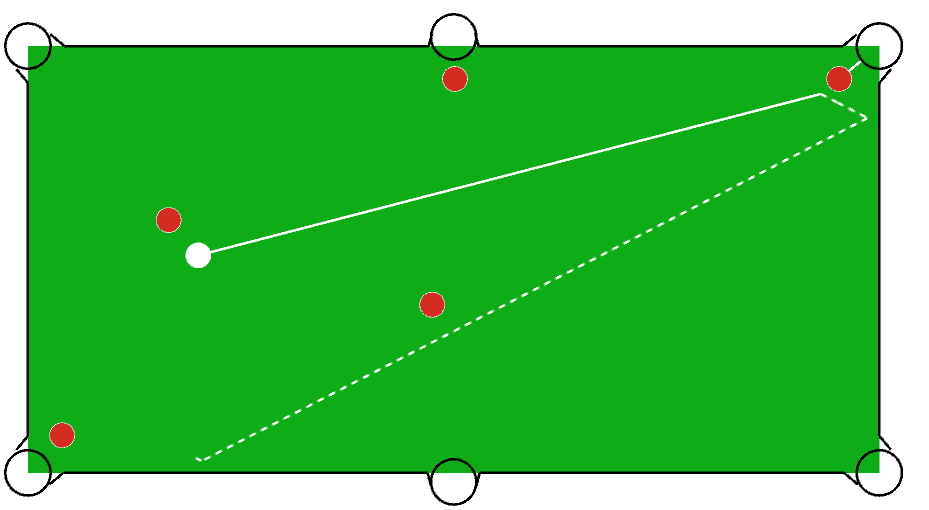
\includegraphics[width=1.0\linewidth]{../common/04_results/resources/simple_search/situation_diverse_solution_velocity_8.PNG}
        \caption{Stoss 8}
        \label{fig:situation_velocity_1_solution_8}
    \end{subfigure}
    \hfill
    \begin{subfigure}[b]{0.3\textwidth}
        \centering
        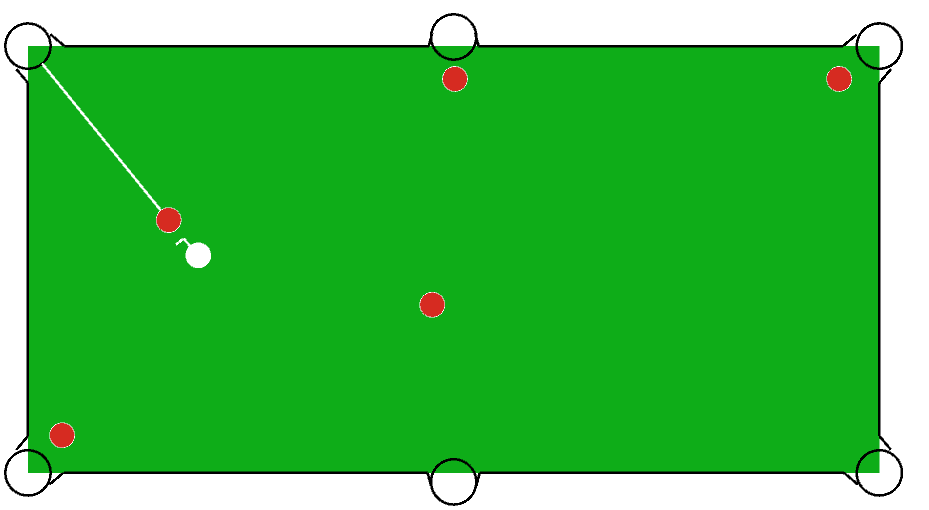
\includegraphics[width=1.0\linewidth]{../common/04_results/resources/simple_search/situation_diverse_solution_velocity_9.PNG}
        \caption{Stoss 9}
        \label{fig:situation_velocity_1_solution_9}
    \end{subfigure}
    \hfill
    \begin{subfigure}[b]{0.3\textwidth}
        \centering
        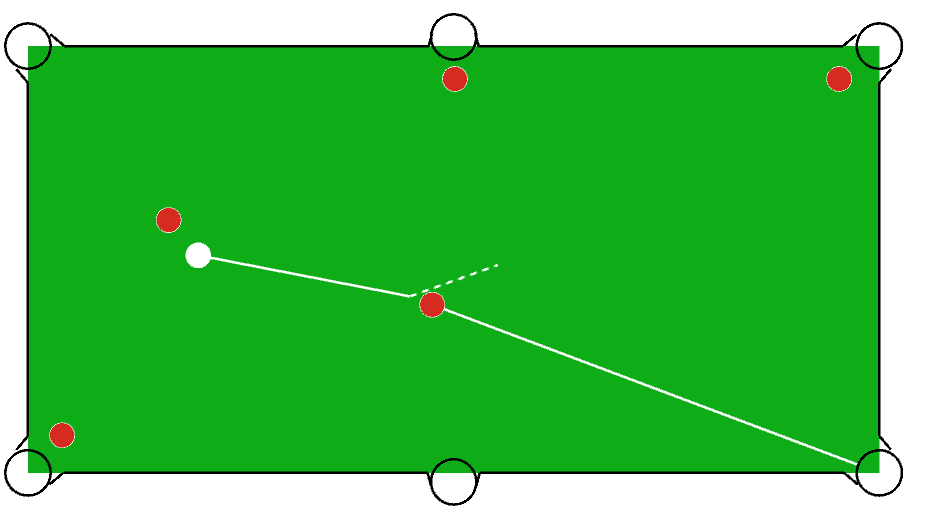
\includegraphics[width=1.0\linewidth]{../common/04_results/resources/simple_search/situation_diverse_solution_velocity_10.PNG}
        \caption{Stoss 10}
        \label{fig:situation_velocity_1_solution_10}
    \end{subfigure}
    \caption{Gefundene Stösse zu Situation 1 nach bewerteter Schwierigkeit aufsteigend mit verschiedenen Startgeschwindigkeiten}
    \label{fig:situation_1_solutions_startgeschwindigkeit}
\end{figure}

Wie zu erwarten war, sieht die Abfolge der Suchresultate nicht wesentlich anders aus wie vorhin.
Bemerkenswerterweise kann eine erhöhte Geschwindigkeit dazu führen, dass ein Stoss,
der einen grösseren Weg und/oder Winkel aufweist, besser bewertet werden kann.
Dies ist z.B. bei Stoss 3 ersichtlich, der besser gewertet wird als Stoss 4 oder bei
Stoss 8, der schwieriger als Stoss 6 und 7 ist. Bei Stoss 8 könnte argumentiert werden, dass die Stärke
in dem Fall keinen grossen Unterschied macht, da die Kugel 2 mit grosser Wahrscheinlichkeit eingelocht werden kann,
jedoch ist generell ein sanftes Billardspiel zu bevorzugen, weswegen die Bewertung in dem Sinne durchaus gerechtfertigt
sein kann.
Die einzelnen Details sind den Tabellen \ref{tab:kosten_erster_vorschlag_ohne_bande_mit_geschwindigkeit},
\ref{tab:kosten_zweiter_vorschlag_ohne_bande_mit_geschwindigkeit}, \ref{tab:kosten_dritter_vorschlag_ohne_bande_mit_geschwindigkeit},
\ref{tab:kosten_vierter_vorschlag_ohne_bande_mit_geschwindigkeit}, \ref{tab:kosten_fuenfter_vorschlag_ohne_bande_mit_geschwindigkeit},
\ref{tab:kosten_sechster_vorschlag_ohne_bande_mit_geschwindigkeit}, \ref{tab:kosten_siebter_vorschlag_ohne_bande_mit_geschwindigkeit},
\ref{tab:kosten_achter_vorschlag_ohne_bande_mit_geschwindigkeit}, \ref{tab:kosten_neunter_vorschlag_ohne_bande_mit_geschwindigkeit}
und \ref{tab:kosten_zehnter_vorschlag_ohne_bande_mit_geschwindigkeit} zu entnehmen.

%[mapToSolution] COST START
%[mapToSolution] cost-search - distance: 0 angle: 0 indirection: 0 sum: 0 cost: 0 previous cost: 0 total cost: 0
%[mapToSolution] cost-search - distance: 0.00284364 angle: 3.93338e-06 indirection: 0 sum: 0.00284757 cost: 284 previous cost: 0 total cost: 284
%[mapToSolution] cost-search - distance: 0.000128041 angle: 7.48246e-05 indirection: 0.5 sum: 0.500203 cost: 50020 previous cost: 284 total cost: 50304
%[mapToSolution] cost-simulation - cost: 21902 previous cost: 50304 total cost: 72206
%[mapToSolution] end cost: 72206
%[mapToSolution] COST END
\begin{table}[h!]
    \rowcolors{1}{\seccolor!10}{\seccolor!10} % Rows with 10% of secondary color
    \begin{tabular}{llrrrr}
        \rowcolor{\seccolor!50}
        Stoss & Segment & Distanzkosten & Winkelkosten & Indirektionskosten & Total (Ganzzahl)\\\bfhmidline
        1          & Weiss - Rot & 0.00012804  & 0.0000748246  & 0.5 & 50020 \\
        1          & Rot - Loch  & 0.00284364  & 0.0000039334  & 0   & 284 \\
        \textbf{1} & \multicolumn{4}{l}{\textbf{Suchkostentotal}}    & \textbf{50304}\\
        1          & Simulation & \multicolumn{4}{r}{21902}\\\bfhmidline
        \multicolumn{5}{l}{\textbf{Gesamttotal}}                     & \textbf{72206}\\
    \end{tabular}
    \caption{Kosten des ersten Vorschlags über einen einfachen Stoss ohne Bandeninteraktion mit vervielfältigter Geschwindigkeit.}
    \label{tab:kosten_erster_vorschlag_ohne_bande_mit_geschwindigkeit}
\end{table}

%[mapToSolution] COST START
%[mapToSolution] cost-search - distance: 0 angle: 0 indirection: 0 sum: 0 cost: 0 previous cost: 0 total cost: 0
%[mapToSolution] cost-search - distance: 0.00284364 angle: 3.93338e-06 indirection: 0 sum: 0.00284757 cost: 284 previous cost: 0 total cost: 284
%[mapToSolution] cost-search - distance: 0.000128041 angle: 7.48246e-05 indirection: 0.5 sum: 0.500203 cost: 50020 previous cost: 284 total cost: 50304
%[mapToSolution] cost-simulation - cost: 24085 previous cost: 50304 total cost: 74389
%[mapToSolution] end cost: 74389
%[mapToSolution] COST END
\begin{table}[h!]
    \rowcolors{1}{\seccolor!10}{\seccolor!10} % Rows with 10% of secondary color
    \begin{tabular}{llrrrr}
        \rowcolor{\seccolor!50}
        Stoss & Segment & Distanzkosten & Winkelkosten & Indirektionskosten & Total (Ganzzahl)\\\bfhmidline
        1          & Weiss - Rot & 0.00012804  & 0.0000748246  & 0.5 & 50020 \\
        1          & Rot - Loch  & 0.00284364  & 0.0000039334  & 0   & 284 \\
        \textbf{1} & \multicolumn{4}{l}{\textbf{Suchkostentotal}}    & \textbf{50304}\\
        1          & Simulation & \multicolumn{4}{r}{24085}\\\bfhmidline
        \multicolumn{5}{l}{\textbf{Gesamttotal}}                     & \textbf{74389}\\
    \end{tabular}
    \caption{Kosten des zweiten Vorschlags über einen einfachen Stoss ohne Bandeninteraktion mit vervielfältigter Geschwindigkeit.}
    \label{tab:kosten_zweiter_vorschlag_ohne_bande_mit_geschwindigkeit}
\end{table}

%[mapToSolution] COST START
%[mapToSolution] cost-search - distance: 0 angle: 0 indirection: 0 sum: 0 cost: 0 previous cost: 0 total cost: 0
%[mapToSolution] cost-search - distance: 0.0029786 angle: 7.36014e-05 indirection: 0 sum: 0.0030522 cost: 305 previous cost: 0 total cost: 305
%[mapToSolution] cost-search - distance: 0.00135804 angle: 0.0237772 indirection: 0.5 sum: 0.525135 cost: 52513 previous cost: 305 total cost: 52818
%[mapToSolution] cost-simulation - cost: 23547 previous cost: 52818 total cost: 76365
%[mapToSolution] end cost: 76365
%[mapToSolution] COST END
\begin{table}[h!]
    \rowcolors{1}{\seccolor!10}{\seccolor!10} % Rows with 10% of secondary color
    \begin{tabular}{llrrrr}
        \rowcolor{\seccolor!50}
        Stoss & Segment & Distanzkosten & Winkelkosten & Indirektionskosten & Total (Ganzzahl)\\\bfhmidline
        1          & Weiss - Rot & 0.001358   & 0.0237772      & 0.5 & 52513 \\
        1          & Rot - Loch  & 0.002979   & 0.0000736      & 0   & 305 \\
        \textbf{1} & \multicolumn{4}{l}{\textbf{Suchkostentotal}}    & \textbf{52818}\\
        1          & Simulation & \multicolumn{4}{r}{23547}\\\bfhmidline
        \multicolumn{5}{l}{\textbf{Gesamttotal}}                     & \textbf{76365}\\
    \end{tabular}
    \caption{Kosten des dritten Vorschlags über einen einfachen Stoss ohne Bandeninteraktion mit vervielfältigter Geschwindigkeit.}
    \label{tab:kosten_dritter_vorschlag_ohne_bande_mit_geschwindigkeit}
\end{table}

%[mapToSolution] COST START
%[mapToSolution] cost-search - distance: 0 angle: 0 indirection: 0 sum: 0 cost: 0 previous cost: 0 total cost: 0
%[mapToSolution] cost-search - distance: 0.00284364 angle: 3.93338e-06 indirection: 0 sum: 0.00284757 cost: 284 previous cost: 0 total cost: 284
%[mapToSolution] cost-search - distance: 0.000128041 angle: 7.48246e-05 indirection: 0.5 sum: 0.500203 cost: 50020 previous cost: 284 total cost: 50304
%[mapToSolution] cost-simulation - cost: 28280 previous cost: 50304 total cost: 78584
%[mapToSolution] end cost: 78584
%[mapToSolution] COST END
\begin{table}[h!]
    \rowcolors{1}{\seccolor!10}{\seccolor!10} % Rows with 10% of secondary color
    \begin{tabular}{llrrrr}
        \rowcolor{\seccolor!50}
        Stoss & Segment & Distanzkosten & Winkelkosten & Indirektionskosten & Total (Ganzzahl)\\\bfhmidline
        1          & Weiss - Rot & 0.00012804   & 0.0000748246     & 0.5 & 50020 \\
        1          & Rot - Loch  & 0.00284364   & 0.0000039334     & 0   & 284 \\
        \textbf{1} & \multicolumn{4}{l}{\textbf{Suchkostentotal}}  & \textbf{50304}\\
        1          & Simulation & \multicolumn{4}{r}{28280}\\\bfhmidline
        \multicolumn{5}{l}{\textbf{Gesamttotal}}                   & \textbf{78584}\\
    \end{tabular}
    \caption{Kosten des vierten Vorschlags über einen einfachen Stoss ohne Bandeninteraktion mit vervielfältigter Geschwindigkeit.}
    \label{tab:kosten_vierter_vorschlag_ohne_bande_mit_geschwindigkeit}
\end{table}

%[mapToSolution] COST START
%[mapToSolution] cost-search - distance: 0 angle: 0 indirection: 0 sum: 0 cost: 0 previous cost: 0 total cost: 0
%[mapToSolution] cost-search - distance: 0.0029786 angle: 7.36014e-05 indirection: 0 sum: 0.0030522 cost: 305 previous cost: 0 total cost: 305
%[mapToSolution] cost-search - distance: 0.00135804 angle: 0.0237772 indirection: 0.5 sum: 0.525135 cost: 52513 previous cost: 305 total cost: 52818
%[mapToSolution] cost-simulation - cost: 26565 previous cost: 52818 total cost: 79383
%[mapToSolution] end cost: 79383
%[mapToSolution] COST END
\begin{table}[h!]
    \rowcolors{1}{\seccolor!10}{\seccolor!10} % Rows with 10% of secondary color
    \begin{tabular}{llrrrr}
        \rowcolor{\seccolor!50}
        Stoss & Segment & Distanzkosten & Winkelkosten & Indirektionskosten & Total (Ganzzahl)\\\bfhmidline
        1          & Weiss - Rot & 0.001358   & 0.0237772          & 0.5 & 52513 \\
        1          & Rot - Loch  & 0.002979   & 0.0000736          & 0   & 305 \\
        \textbf{1} & \multicolumn{4}{l}{\textbf{Suchkostentotal}}  & \textbf{52818}\\
        1          & Simulation & \multicolumn{4}{r}{26565}\\\bfhmidline
        \multicolumn{5}{l}{\textbf{Gesamttotal}}                   & \textbf{79383}\\
    \end{tabular}
    \caption{Kosten des fünften Vorschlags über einen einfachen Stoss ohne Bandeninteraktion mit vervielfältigter Geschwindigkeit.}
    \label{tab:kosten_fuenfter_vorschlag_ohne_bande_mit_geschwindigkeit}
\end{table}

%[mapToSolution] COST START
%[mapToSolution] cost-search - distance: 0 angle: 0 indirection: 0 sum: 0 cost: 0 previous cost: 0 total cost: 0
%[mapToSolution] cost-search - distance: 0.0552051 angle: 9.28795e-05 indirection: 0 sum: 0.055298 cost: 5529 previous cost: 0 total cost: 5529
%[mapToSolution] cost-search - distance: 3.0656e-05 angle: 2.01923e-06 indirection: 0.5 sum: 0.500033 cost: 50003 previous cost: 5529 total cost: 55532
%[mapToSolution] cost-simulation - cost: 24388 previous cost: 55532 total cost: 79920
%[mapToSolution] end cost: 79920
%[mapToSolution] COST END
\begin{table}[h!]
    \rowcolors{1}{\seccolor!10}{\seccolor!10} % Rows with 10% of secondary color
    \begin{tabular}{llrrrr}
        \rowcolor{\seccolor!50}
        Stoss & Segment & Distanzkosten & Winkelkosten & Indirektionskosten & Total (Ganzzahl)\\\bfhmidline
        1          & Weiss - Rot & 0.0000307  & 0.0000020192       & 0.5 & 50003 \\
        1          & Rot - Loch  & 0.055205   & 0.0000928795       & 0   & 5529 \\
        \textbf{1} & \multicolumn{4}{l}{\textbf{Suchkostentotal}}  & \textbf{55532}\\
        1          & Simulation & \multicolumn{4}{r}{24388}\\\bfhmidline
        \multicolumn{5}{l}{\textbf{Gesamttotal}}                   & \textbf{79920}\\
    \end{tabular}
    \caption{Kosten des sechsten Vorschlags über einen einfachen Stoss ohne Bandeninteraktion mit vervielfältigter Geschwindigkeit.}
    \label{tab:kosten_sechster_vorschlag_ohne_bande_mit_geschwindigkeit}
\end{table}

%[mapToSolution] COST START
%[mapToSolution] cost-search - distance: 0 angle: 0 indirection: 0 sum: 0 cost: 0 previous cost: 0 total cost: 0
%[mapToSolution] cost-search - distance: 0.0552051 angle: 9.28795e-05 indirection: 0 sum: 0.055298 cost: 5529 previous cost: 0 total cost: 5529
%[mapToSolution] cost-search - distance: 3.0656e-05 angle: 2.01923e-06 indirection: 0.5 sum: 0.500033 cost: 50003 previous cost: 5529 total cost: 55532
%[mapToSolution] cost-simulation - cost: 27115 previous cost: 55532 total cost: 82647
%[mapToSolution] end cost: 82647
%[mapToSolution] COST END
\begin{table}[h!]
    \rowcolors{1}{\seccolor!10}{\seccolor!10} % Rows with 10% of secondary color
    \begin{tabular}{llrrrr}
        \rowcolor{\seccolor!50}
        Stoss & Segment & Distanzkosten & Winkelkosten & Indirektionskosten & Total (Ganzzahl)\\\bfhmidline
        1          & Weiss - Rot & 0.0000307   & 0.0000020192       & 0.5 & 50003 \\
        1          & Rot - Loch  & 0.0552051   & 0.0000928795       & 0   & 5529 \\
        \textbf{1} & \multicolumn{4}{l}{\textbf{Suchkostentotal}}  & \textbf{55532}\\
        1          & Simulation & \multicolumn{4}{r}{27115}\\\bfhmidline
        \multicolumn{5}{l}{\textbf{Gesamttotal}}                   & \textbf{82647}\\
    \end{tabular}
    \caption{Kosten des siebten Vorschlags über einen einfachen Stoss ohne Bandeninteraktion mit vervielfältigter Geschwindigkeit.}
    \label{tab:kosten_siebter_vorschlag_ohne_bande_mit_geschwindigkeit}
\end{table}

%[mapToSolution] COST START
%[mapToSolution] cost-search - distance: 0 angle: 0 indirection: 0 sum: 0 cost: 0 previous cost: 0 total cost: 0
%[mapToSolution] cost-search - distance: 0.0029786 angle: 7.36014e-05 indirection: 0 sum: 0.0030522 cost: 305 previous cost: 0 total cost: 305
%[mapToSolution] cost-search - distance: 0.00135804 angle: 0.0237772 indirection: 0.5 sum: 0.525135 cost: 52513 previous cost: 305 total cost: 52818
%[mapToSolution] cost-simulation - cost: 31695 previous cost: 52818 total cost: 84513
%[mapToSolution] end cost: 84513
%[mapToSolution] COST END
\begin{table}[h!]
    \rowcolors{1}{\seccolor!10}{\seccolor!10} % Rows with 10% of secondary color
    \begin{tabular}{llrrrr}
        \rowcolor{\seccolor!50}
        Stoss & Segment & Distanzkosten & Winkelkosten & Indirektionskosten & Total (Ganzzahl)\\\bfhmidline
        1          & Weiss - Rot & 0.001358    & 0.0237772          & 0.5 & 52513 \\
        1          & Rot - Loch  & 0.0029786   & 0.0000736014       & 0   & 305 \\
        \textbf{1} & \multicolumn{4}{l}{\textbf{Suchkostentotal}}  & \textbf{52818}\\
        1          & Simulation & \multicolumn{4}{r}{31695}\\\bfhmidline
        \multicolumn{5}{l}{\textbf{Gesamttotal}}                   & \textbf{84513}\\
    \end{tabular}
    \caption{Kosten des achten Vorschlags über einen einfachen Stoss ohne Bandeninteraktion mit vervielfältigter Geschwindigkeit.}
    \label{tab:kosten_achter_vorschlag_ohne_bande_mit_geschwindigkeit}
\end{table}

%[mapToSolution] COST START
%[mapToSolution] cost-search - distance: 0 angle: 0 indirection: 0 sum: 0 cost: 0 previous cost: 0 total cost: 0
%[mapToSolution] cost-search - distance: 0.0552051 angle: 9.28795e-05 indirection: 0 sum: 0.055298 cost: 5529 previous cost: 0 total cost: 5529
%[mapToSolution] cost-search - distance: 3.0656e-05 angle: 2.01923e-06 indirection: 0.5 sum: 0.500033 cost: 50003 previous cost: 5529 total cost: 55532
%[mapToSolution] cost-simulation - cost: 32064 previous cost: 55532 total cost: 87596
%[mapToSolution] end cost: 87596
%[mapToSolution] COST END
\begin{table}[h!]
    \rowcolors{1}{\seccolor!10}{\seccolor!10} % Rows with 10% of secondary color
    \begin{tabular}{llrrrr}
        \rowcolor{\seccolor!50}
        Stoss & Segment & Distanzkosten & Winkelkosten & Indirektionskosten & Total (Ganzzahl)\\\bfhmidline
        1          & Weiss - Rot & 0.0000307    & 0.00000201923      & 0.5 & 50003 \\
        1          & Rot - Loch  & 0.0552051    & 0.0000928795       & 0   & 5529 \\
        \textbf{1} & \multicolumn{4}{l}{\textbf{Suchkostentotal}}  & \textbf{55532}\\
        1          & Simulation & \multicolumn{4}{r}{32064}\\\bfhmidline
        \multicolumn{5}{l}{\textbf{Gesamttotal}}                   & \textbf{87596}\\
    \end{tabular}
    \caption{Kosten des neunten Vorschlags über einen einfachen Stoss ohne Bandeninteraktion mit vervielfältigter Geschwindigkeit.}
    \label{tab:kosten_neunter_vorschlag_ohne_bande_mit_geschwindigkeit}
\end{table}

%[mapToSolution] COST START
%[mapToSolution] cost-search - distance: 0 angle: 0 indirection: 0 sum: 0 cost: 0 previous cost: 0 total cost: 0
%[mapToSolution] cost-search - distance: 0.251514 angle: 0.0224747 indirection: 0 sum: 0.273988 cost: 27398 previous cost: 0 total cost: 27398
%[mapToSolution] cost-search - distance: 0.0129086 angle: 0.000592332 indirection: 0.5 sum: 0.513501 cost: 51350 previous cost: 27398 total cost: 78748
%[mapToSolution] cost-simulation - cost: 35872 previous cost: 78748 total cost: 114620
%[mapToSolution] end cost: 114620
%[mapToSolution] COST END
\begin{table}[h!]
    \rowcolors{1}{\seccolor!10}{\seccolor!10} % Rows with 10% of secondary color
    \begin{tabular}{llrrrr}
        \rowcolor{\seccolor!50}
        Stoss & Segment & Distanzkosten & Winkelkosten & Indirektionskosten & Total (Ganzzahl)\\\bfhmidline
        1          & Weiss - Rot & 0.012909     & 0.0005923       & 0.5 & 51350 \\
        1          & Rot - Loch  & 0.251514     & 0.0224747       & 0   & 27398 \\
        \textbf{1} & \multicolumn{4}{l}{\textbf{Suchkostentotal}}  & \textbf{78748}\\
        1          & Simulation & \multicolumn{4}{r}{35872}\\\bfhmidline
        \multicolumn{5}{l}{\textbf{Gesamttotal}}                   & \textbf{114620}\\
    \end{tabular}
    \caption{Kosten des zehnten Vorschlags über einen einfachen Stoss ohne Bandeninteraktion mit vervielfältigter Geschwindigkeit.}
    \label{tab:kosten_zehnter_vorschlag_ohne_bande_mit_geschwindigkeit}
\end{table}

\clearpage
\subsection{Die einfache Suche - mit Bandenkollisionen}
In diesem Fall werden verschiedene Startgeschwindigkeiten nicht berücksichtigt, jedoch wird das Bandenspiel zugelassen.
Auch hier sollten sich die Resultate nicht wesentlich zur einfachen Suche in Kapitel \ref{kap:suche:die_einfache_suche} ändern.
Ein Unterschied ist vor allem gegen Ende bei Stoss 6 und 7 zu erwarten, so wird eventuell eher ein Spiel über eine Bande berücksichtigt
als der starke Stoss 7 oder der indirekte Stoss 6.

In Abbildung \ref{fig:situation_1_solutions_bande} sind die Resultate in aufsteigender Schwierigkeit gegeben.

\begin{figure}[h!]
    \centering
    \begin{subfigure}[b]{0.3\textwidth}
        \centering
        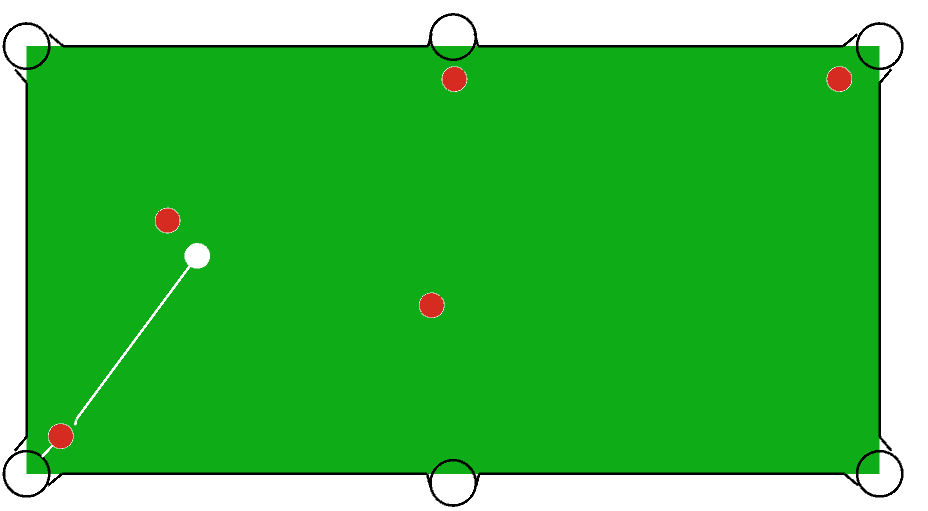
\includegraphics[width=1.0\linewidth]{../common/04_results/resources/simple_search/situation_diverse_solution_rail_1.PNG}
        \caption{Stoss 1}
        \label{fig:situation_rail_1_solution_1}
    \end{subfigure}
    \hfill
    \begin{subfigure}[b]{0.3\textwidth}
        \centering
        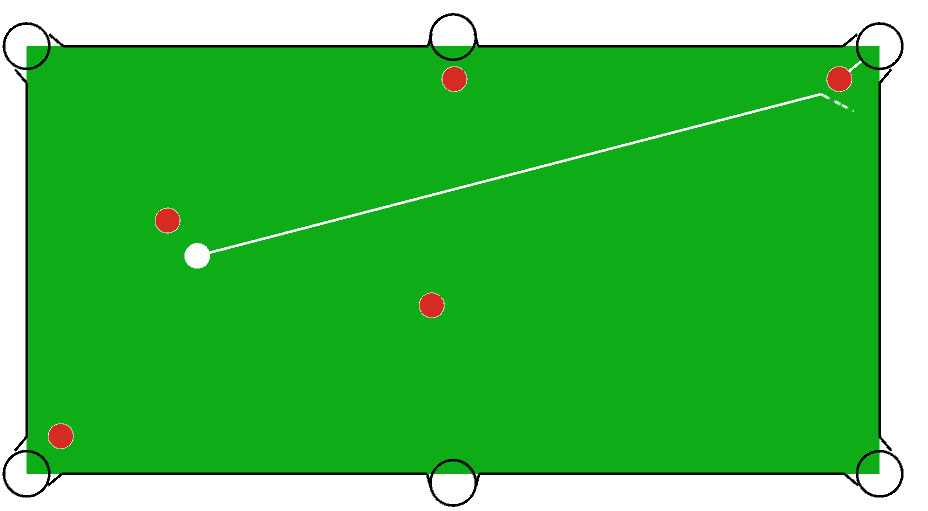
\includegraphics[width=1.0\linewidth]{../common/04_results/resources/simple_search/situation_diverse_solution_rail_2.PNG}
        \caption{Stoss 2}
        \label{fig:situation_rail_1_solution_2}
    \end{subfigure}
    \hfill
    \begin{subfigure}[b]{0.3\textwidth}
        \centering
        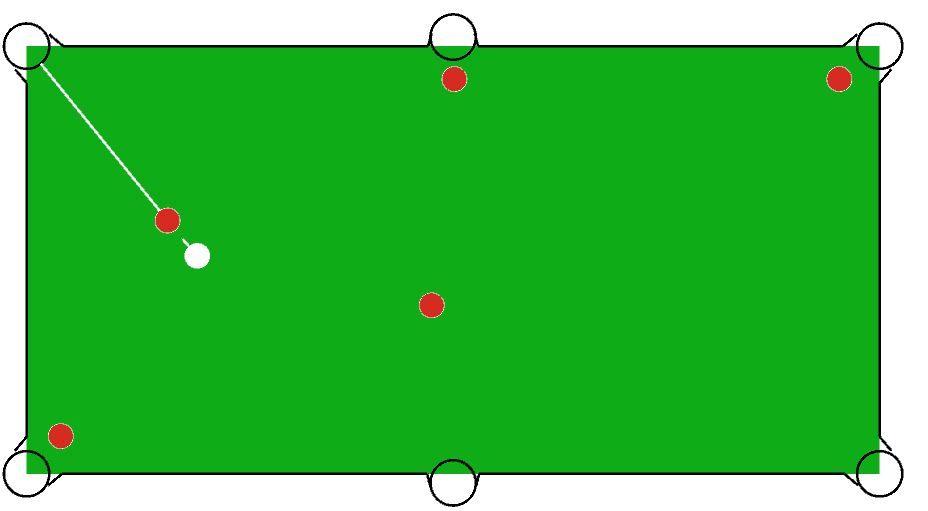
\includegraphics[width=1.0\linewidth]{../common/04_results/resources/simple_search/situation_diverse_solution_rail_3.PNG}
        \caption{Stoss 3}
        \label{fig:situation_rail_1_solution_3}
    \end{subfigure}
    \hfill
    \begin{subfigure}[b]{0.3\textwidth}
        \centering
        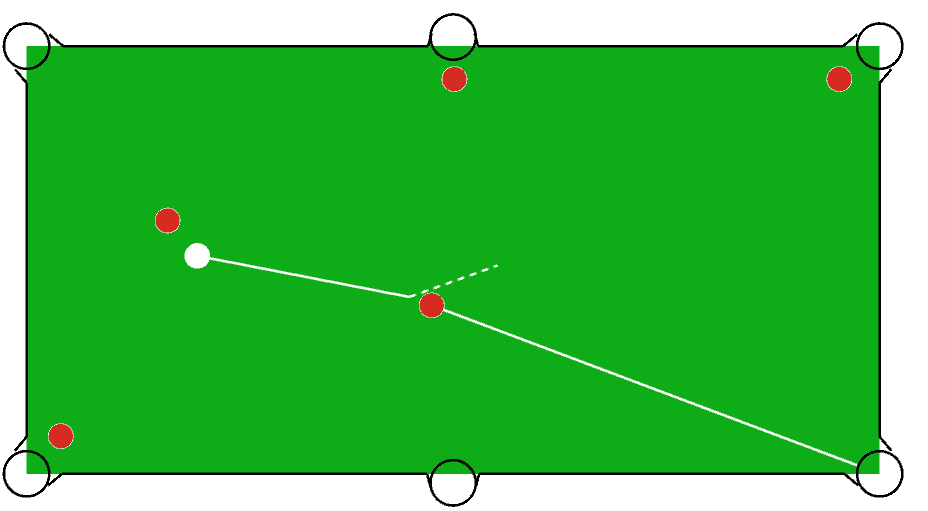
\includegraphics[width=1.0\linewidth]{../common/04_results/resources/simple_search/situation_diverse_solution_rail_4.PNG}
        \caption{Stoss 4}
        \label{fig:situation_rail_1_solution_4}
    \end{subfigure}
    \hfill
    \begin{subfigure}[b]{0.3\textwidth}
        \centering
        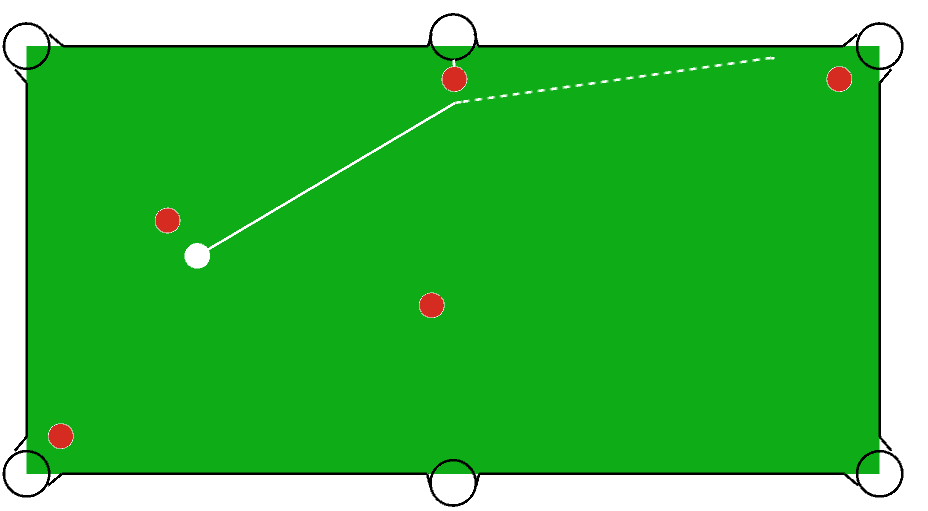
\includegraphics[width=1.0\linewidth]{../common/04_results/resources/simple_search/situation_diverse_solution_rail_5.PNG}
        \caption{Stoss 5}
        \label{fig:situation_rail_1_solution_5}
    \end{subfigure}
    \hfill
    \begin{subfigure}[b]{0.3\textwidth}
        \centering
        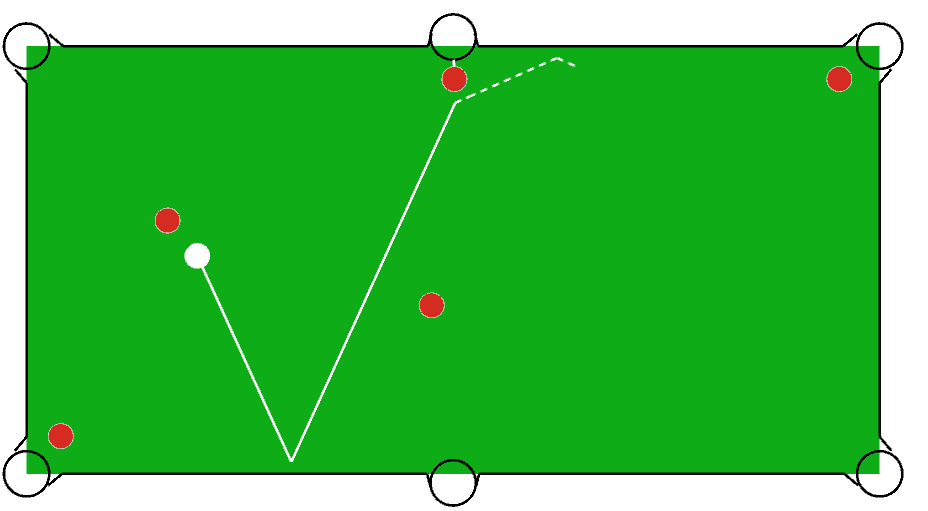
\includegraphics[width=1.0\linewidth]{../common/04_results/resources/simple_search/situation_diverse_solution_rail_6.PNG}
        \caption{Stoss 6}
        \label{fig:situation_rail_1_solution_6}
    \end{subfigure}
    \hfill
    \begin{subfigure}[b]{0.3\textwidth}
        \centering
        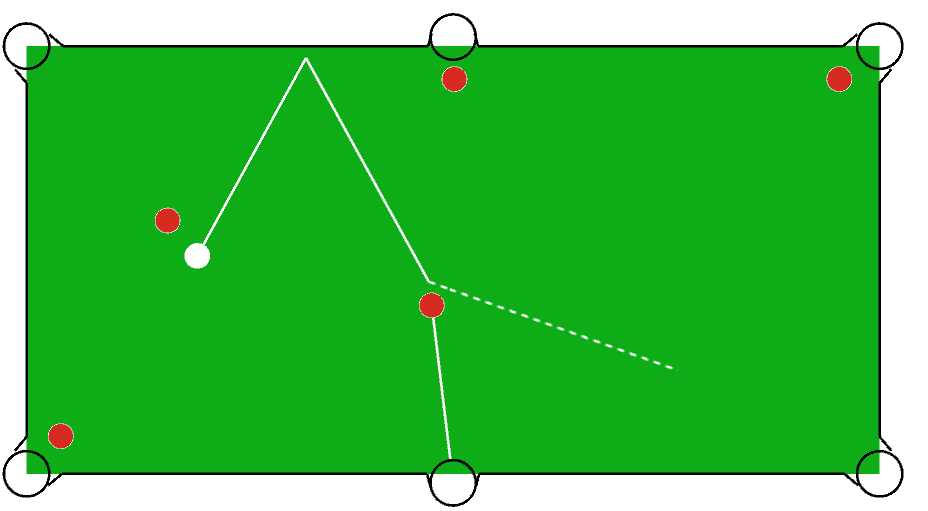
\includegraphics[width=1.0\linewidth]{../common/04_results/resources/simple_search/situation_diverse_solution_rail_7.PNG}
        \caption{Stoss 7}
        \label{fig:situation_rail_1_solution_7}
    \end{subfigure}
    \hfill
    \begin{subfigure}[b]{0.3\textwidth}
        \centering
        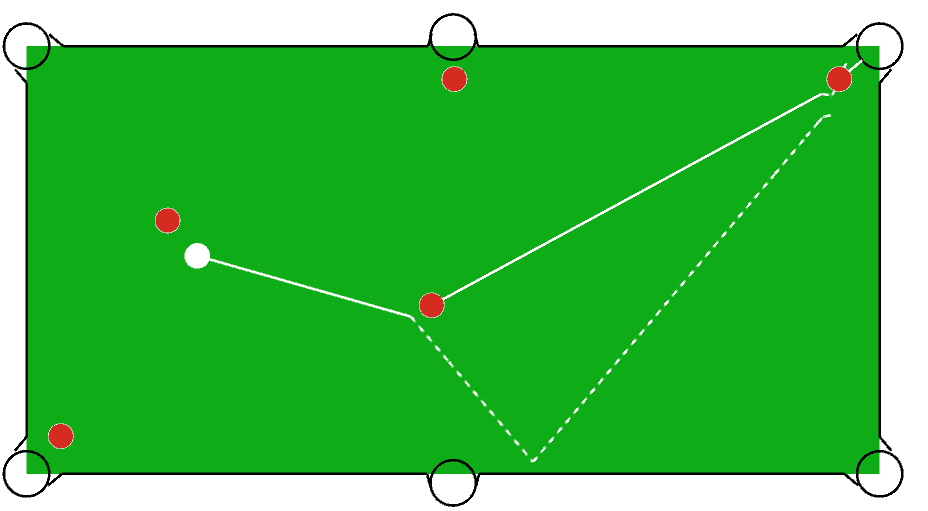
\includegraphics[width=1.0\linewidth]{../common/04_results/resources/simple_search/situation_diverse_solution_rail_8.PNG}
        \caption{Stoss 8}
        \label{fig:situation_rail_1_solution_8}
    \end{subfigure}
    \hfill
    \begin{subfigure}[b]{0.3\textwidth}
        \centering
        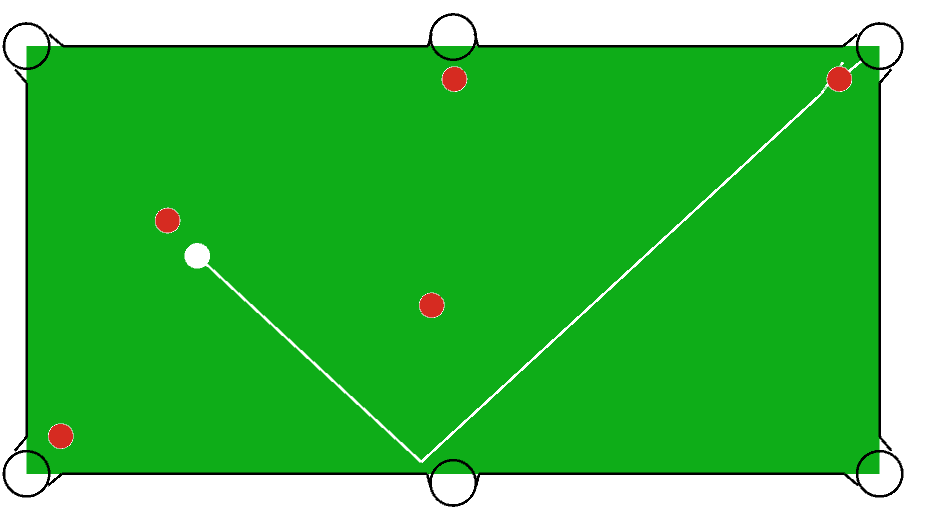
\includegraphics[width=1.0\linewidth]{../common/04_results/resources/simple_search/situation_diverse_solution_rail_9.PNG}
        \caption{Stoss 9}
        \label{fig:situation_rail_1_solution_9}
    \end{subfigure}
    \hfill
    \begin{subfigure}[b]{0.3\textwidth}
        \centering
        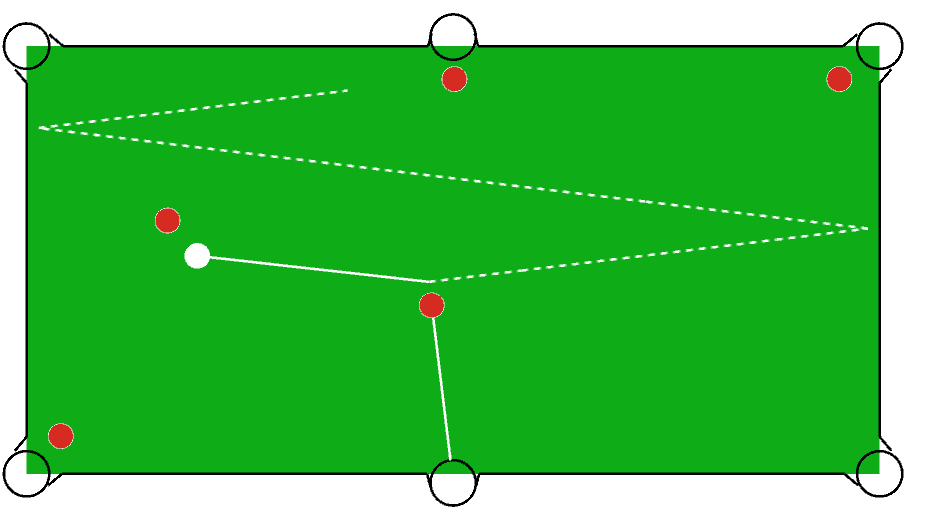
\includegraphics[width=1.0\linewidth]{../common/04_results/resources/simple_search/situation_diverse_solution_rail_10.PNG}
        \caption{Stoss 10}
        \label{fig:situation_rail_1_solution_10}
    \end{subfigure}
    \caption{Gefundene Stösse zu Situation 1 nach bewerteter Schwierigkeit aufsteigend mit Berücksichtigung der Banden}
    \label{fig:situation_1_solutions_bande}
\end{figure}

Bis zu Stoss 5 gibt es keine Änderungen der Vorschläge. Bei Stoss 6 wird
anstelle des indirekten Stosses auf Kugel 2 in Kapitel \ref{kap:suche:die_einfache_suche} jedoch eine Lösung über
die untere Bande auf Kugel 3 empfohlen. Dies macht Sinn, da das Spiel über
die untere Bande einerseits direkter ist und andererseits eine ähnliche Distanz
mit kleineren Winkeln vorliegt. Zudem liegt die Kugel 3 näher am Loch als die Kugel 2.

Stoss 7 schlägt eine ähnliche Lösung wie Stoss 6 vor, jedoch über die obere Bande auf die Kugel 5, die im
mittleren unteren Loch versenkt wird. Auch dies ist eine direktere Lösung mit kleineren Distanzen
als der Stoss 6 aus Kapitel \ref{kap:suche:die_einfache_suche}, er wird aber auch schlechter als Stoss 6 dieses Kapitels
gewertet, da die Kugel 5 einen längeren Weg zum Loch zurücklegen muss, was die Wahrscheinlichkeit
eines akkumulierten Fehlers erhöht.

Stoss 8 entspricht nun dem Stoss 6 aus Kapitel \ref{kap:suche:die_einfache_suche}. Dieser reiht sich vor
dem Stoss 9 dieses Kapitels ein, wo es ebenfalls um das Versenken der Kugel 2 geht. Da die Distanzen
zwischen den Kugeln kleiner sind und die Winkel ungefähr gleich gross, wird der indirekte Stoss
über eine Kugel bevorzugt.

Abschliessend zeigt Stoss 10 das direkte Versenken der Kugel 5 im mittleren unteren Loch.
Da der Winkel und die Startgeschwindigkeit sehr gross sind, ist die hohe Schwierigkeit durchaus nachzuvollziehen.

Die detaillierte Aufführung der Kosten jedes Stosses sind in den Tabellen \ref{tab:kosten_vorschlag_mit_bande_1},
\ref{tab:kosten_vorschlag_mit_bande_2}, \ref{tab:kosten_vorschlag_mit_bande_3}, \ref{tab:kosten_vorschlag_mit_bande_4},
\ref{tab:kosten_vorschlag_mit_bande_5}, \ref{tab:kosten_vorschlag_mit_bande_6}, \ref{tab:kosten_vorschlag_mit_bande_7},
\ref{tab:kosten_vorschlag_mit_bande_8}, \ref{tab:kosten_vorschlag_mit_bande_9} und \ref{tab:kosten_vorschlag_mit_bande_10}
aufgeführt.

%%[mapToSolution] COST START
%%[mapToSolution] cost-search - distance: 0 angle: 0 indirection: 0 sum: 0 cost: 0 previous cost: 0 total cost: 0
%%[mapToSolution] cost-search - distance: 0.00284364 angle: 3.93338e-06 indirection: 0 sum: 0.00284757 cost: 284 previous cost: 0 total cost: 284
%%[mapToSolution] cost-search - distance: 0.000128041 angle: 7.48246e-05 indirection: 0.5 sum: 0.500203 cost: 50020 previous cost: 284 total cost: 50304
%%[mapToSolution] cost-simulation - cost: 21902 previous cost: 50304 total cost: 72206
%%[mapToSolution] end cost: 72206
%%[mapToSolution] COST END

\begin{table}[h!]
    \rowcolors{1}{\seccolor!10}{\seccolor!10} % Rows with 10% of secondary color
    \begin{tabular}{llrrrr}
        \rowcolor{\seccolor!50}
        Stoss & Segment & Distanzkosten & Winkelkosten & Indirektionskosten & Total (Ganzzahl)\\\bfhmidline
        2          & Weiss - Rot & 0.000128041   & 0.0000748              & 0.5   & 50020 \\
        2          & Rot - Loch  & 0.00284364    & 0.000003933            & 0     & 284 \\
        \textbf{2} & \multicolumn{4}{l}{\textbf{Suchkostentotal}}    & \textbf{50304}\\
        2          & Simulation & \multicolumn{4}{r}{21902}\\\bfhmidline
        \multicolumn{5}{l}{\textbf{Gesamttotal}}                     & \textbf{72206}\\
    \end{tabular}
    \caption{Detaillierte Kosten von Stoss 1 aus Abbildung \ref{fig:situation_1_solutions_bande}.}
    \label{tab:kosten_vorschlag_mit_bande_1}
\end{table}

%%[mapToSolution] COST START
%%[mapToSolution] cost-search - distance: 0 angle: 0 indirection: 0 sum: 0 cost: 0 previous cost: 0 total cost: 0
%%[mapToSolution] cost-search - distance: 0.0029786 angle: 7.36014e-05 indirection: 0 sum: 0.0030522 cost: 305 previous cost: 0 total cost: 305
%%[mapToSolution] cost-search - distance: 0.00135804 angle: 0.0237772 indirection: 0.5 sum: 0.525135 cost: 52513 previous cost: 305 total cost: 52818
%%[mapToSolution] cost-simulation - cost: 23547 previous cost: 52818 total cost: 76365
%%[mapToSolution] end cost: 76365
%%[mapToSolution] COST END

\begin{table}[h!]
    \rowcolors{1}{\seccolor!10}{\seccolor!10} % Rows with 10% of secondary color
    \begin{tabular}{llrrrr}
        \rowcolor{\seccolor!50}
        Stoss & Segment & Distanzkosten & Winkelkosten & Indirektionskosten & Total (Ganzzahl)\\\bfhmidline
        2          & Weiss - Rot & 0.00135804   & 0.0237772              & 0.5   & 52513 \\
        2          & Rot - Loch  & 0.0029786    & 0.0000736014           & 0     & 305 \\
        \textbf{2} & \multicolumn{4}{l}{\textbf{Suchkostentotal}}    & \textbf{52818}\\
        2          & Simulation & \multicolumn{4}{r}{23547}\\\bfhmidline
        \multicolumn{5}{l}{\textbf{Gesamttotal}}                     & \textbf{76365}\\
    \end{tabular}
    \caption{Detaillierte Kosten von Stoss 2 aus Abbildung \ref{fig:situation_1_solutions_bande}.}
    \label{tab:kosten_vorschlag_mit_bande_2}
\end{table}

%%[mapToSolution] COST START
%%[mapToSolution] cost-search - distance: 0 angle: 0 indirection: 0 sum: 0 cost: 0 previous cost: 0 total cost: 0
%%[mapToSolution] cost-search - distance: 0.0552051 angle: 9.28795e-05 indirection: 0 sum: 0.055298 cost: 5529 previous cost: 0 total cost: 5529
%%[mapToSolution] cost-search - distance: 3.0656e-05 angle: 2.01923e-06 indirection: 0.5 sum: 0.500033 cost: 50003 previous cost: 5529 total cost: 55532
%%[mapToSolution] cost-simulation - cost: 24388 previous cost: 55532 total cost: 79920
%%[mapToSolution] end cost: 79920
%%[mapToSolution] COST END

\begin{table}[h!]
    \rowcolors{1}{\seccolor!10}{\seccolor!10} % Rows with 10% of secondary color
    \begin{tabular}{llrrrr}
        \rowcolor{\seccolor!50}
        Stoss & Segment & Distanzkosten & Winkelkosten & Indirektionskosten & Total (Ganzzahl)\\\bfhmidline
        3          & Weiss - Rot & 0.00003066   & 0.0000020193           & 0.5   & 50003 \\
        3          & Rot - Loch  & 0.0552051    & 0.0000928795           & 0     & 5529 \\
        \textbf{3} & \multicolumn{4}{l}{\textbf{Suchkostentotal}}    & \textbf{55532}\\
        3          & Simulation & \multicolumn{4}{r}{24388}\\\bfhmidline
        \multicolumn{5}{l}{\textbf{Gesamttotal}}                     & \textbf{79920}\\
    \end{tabular}
    \caption{Detaillierte Kosten von Stoss 3 aus Abbildung \ref{fig:situation_1_solutions_bande}.}
    \label{tab:kosten_vorschlag_mit_bande_3}
\end{table}

%%[mapToSolution] COST START
%%[mapToSolution] cost-search - distance: 0 angle: 0 indirection: 0 sum: 0 cost: 0 previous cost: 0 total cost: 0
%%[mapToSolution] cost-search - distance: 0.251514 angle: 0.0224747 indirection: 0 sum: 0.273988 cost: 27398 previous cost: 0 total cost: 27398
%%[mapToSolution] cost-search - distance: 0.0129086 angle: 0.000592332 indirection: 0.5 sum: 0.513501 cost: 51350 previous cost: 27398 total cost: 78748
%%[mapToSolution] cost-simulation - cost: 35872 previous cost: 78748 total cost: 114620
%%[mapToSolution] end cost: 114620
%%[mapToSolution] COST END

\begin{table}[h!]
    \rowcolors{1}{\seccolor!10}{\seccolor!10} % Rows with 10% of secondary color
    \begin{tabular}{llrrrr}
        \rowcolor{\seccolor!50}
        Stoss & Segment & Distanzkosten & Winkelkosten & Indirektionskosten & Total (Ganzzahl)\\\bfhmidline
        4          & Weiss - Rot & 0.0129086   & 0.000592332         & 0.5 & 51350 \\
        4          & Rot - Loch  & 0.251514    & 0.0224747           & 0     & 27398 \\
        \textbf{4} & \multicolumn{4}{l}{\textbf{Suchkostentotal}}    & \textbf{78748}\\
        4          & Simulation & \multicolumn{4}{r}{35872}\\\bfhmidline
        \multicolumn{5}{l}{\textbf{Gesamttotal}}                     & \textbf{114620}\\
    \end{tabular}
    \caption{Detaillierte Kosten von Stoss 4 aus Abbildung \ref{fig:situation_1_solutions_bande}.}
    \label{tab:kosten_vorschlag_mit_bande_4}
\end{table}

%%[mapToSolution] COST START
%%[mapToSolution] cost-search - distance: 0 angle: 0 indirection: 0 sum: 0 cost: 0 previous cost: 0 total cost: 0
%%[mapToSolution] cost-search - distance: 0.00194371 angle: 7.48391e-07 indirection: 0 sum: 0.00194446 cost: 194 previous cost: 0 total cost: 194
%%[mapToSolution] cost-search - distance: 0.000191993 angle: 0.525736 indirection: 0.5 sum: 1.02593 cost: 102592 previous cost: 194 total cost: 102786
%%[mapToSolution] cost-simulation - cost: 45576 previous cost: 102786 total cost: 148362
%%[mapToSolution] end cost: 148362
%%[mapToSolution] COST END

\begin{table}[h!]
    \rowcolors{1}{\seccolor!10}{\seccolor!10} % Rows with 10% of secondary color
    \begin{tabular}{llrrrr}
        \rowcolor{\seccolor!50}
        Stoss & Segment & Distanzkosten & Winkelkosten & Indirektionskosten & Total (Ganzzahl)\\\bfhmidline
        5          & Weiss - Rot & 0.000191993   & 0.525736          & 0.5 & 102592 \\
        5          & Rot - Loch  & 0.00194371    & 0.000000748391    & 0     & 194 \\
        \textbf{5} & \multicolumn{4}{l}{\textbf{Suchkostentotal}}    & \textbf{102786}\\
        5          & Simulation & \multicolumn{4}{r}{45576}\\\bfhmidline
        \multicolumn{5}{l}{\textbf{Gesamttotal}}                     & \textbf{148362}\\
    \end{tabular}
    \caption{Detaillierte Kosten von Stoss 5 aus Abbildung \ref{fig:situation_1_solutions_bande}.}
    \label{tab:kosten_vorschlag_mit_bande_5}
\end{table}

%%[mapToSolution] COST START
%%[mapToSolution] cost-search - distance: 0 angle: 0 indirection: 0 sum: 0 cost: 0 previous cost: 0 total cost: 0
%%[mapToSolution] cost-search - distance: 0.00194371 angle: 7.48391e-07 indirection: 0 sum: 0.00194446 cost: 194 previous cost: 0 total cost: 194
%%[mapToSolution] cost-search - distance: 0.000442139 angle: 0.0530682 indirection: 1.16667 sum: 1.22018 cost: 122017 previous cost: 194 total cost: 122211
%%[mapToSolution] cost-simulation - cost: 59446 previous cost: 122211 total cost: 181657
%%[mapToSolution] end cost: 181657
%%[mapToSolution] COST END

\begin{table}[h!]
    \rowcolors{1}{\seccolor!10}{\seccolor!10} % Rows with 10% of secondary color
    \begin{tabular}{llrrrr}
        \rowcolor{\seccolor!50}
        Stoss & Segment & Distanzkosten & Winkelkosten & Indirektionskosten & Total (Ganzzahl)\\\bfhmidline
        6          & Weiss - Rot & 0.000442139   & 0.0530682       & 1.167 & 122017 \\
        6          & Rot - Loch  & 0.00194371    & 0.000000748391       & 0     & 194 \\
        \textbf{6} & \multicolumn{4}{l}{\textbf{Suchkostentotal}}    & \textbf{122211}\\
        6          & Simulation & \multicolumn{4}{r}{59446}\\\bfhmidline
        \multicolumn{5}{l}{\textbf{Gesamttotal}}                     & \textbf{181657}\\
    \end{tabular}
    \caption{Detaillierte Kosten von Stoss 6 aus Abbildung \ref{fig:situation_1_solutions_bande}.}
    \label{tab:kosten_vorschlag_mit_bande_6}
\end{table}

%%[mapToSolution] COST START
%%[mapToSolution] cost-search - distance: 0 angle: 0 indirection: 0 sum: 0 cost: 0 previous cost: 0 total cost: 0
%%[mapToSolution] cost-search - distance: 0.0351119 angle: 0.000154641 indirection: 0 sum: 0.0352666 cost: 3526 previous cost: 0 total cost: 3526
%%[mapToSolution] cost-search - distance: 0.00447887 angle: 0.0568589 indirection: 1.16667 sum: 1.228 cost: 122800 previous cost: 3526 total cost: 126326
%%[mapToSolution] cost-simulation - cost: 63750 previous cost: 126326 total cost: 190076
%%[mapToSolution] end cost: 190076
%%[mapToSolution] COST END

\begin{table}[h!]
    \rowcolors{1}{\seccolor!10}{\seccolor!10} % Rows with 10% of secondary color
    \begin{tabular}{llrrrr}
        \rowcolor{\seccolor!50}
        Stoss & Segment & Distanzkosten & Winkelkosten & Indirektionskosten & Total (Ganzzahl)\\\bfhmidline
        7          & Weiss - Rot & 0.00447887   & 0.0568589       & 1.167 & 122800 \\
        7          & Rot - Loch  & 0.0351119    & 0.0001546       & 0     & 3526 \\
        \textbf{7} & \multicolumn{4}{l}{\textbf{Suchkostentotal}}    & \textbf{126326}\\
        7          & Simulation & \multicolumn{4}{r}{63750}\\\bfhmidline
        \multicolumn{5}{l}{\textbf{Gesamttotal}}                     & \textbf{190076}\\
    \end{tabular}
    \caption{Detaillierte Kosten von Stoss 7 aus Abbildung \ref{fig:situation_1_solutions_bande}.}
    \label{tab:kosten_vorschlag_mit_bande_7}
\end{table}

%%[mapToSolution] COST START
%%[mapToSolution] cost-search - distance: 0 angle: 0 indirection: 0 sum: 0 cost: 0 previous cost: 0 total cost: 0
%%[mapToSolution] cost-search - distance: 0.0029786 angle: 7.36014e-05 indirection: 0 sum: 0.0030522 cost: 305 previous cost: 0 total cost: 305
%%[mapToSolution] cost-search - distance: 0.215404 angle: 0.000932547 indirection: 0.5 sum: 0.716337 cost: 71633 previous cost: 305 total cost: 71938
%%[mapToSolution] cost-search - distance: 0.0116657 angle: 0.197609 indirection: 0.5 sum: 0.709275 cost: 70927 previous cost: 71938 total cost: 142865
%%[mapToSolution] cost-simulation - cost: 68868 previous cost: 142865 total cost: 211733
%%[mapToSolution] end cost: 211733
%%[mapToSolution] COST END

\begin{table}[h!]
    \rowcolors{1}{\seccolor!10}{\seccolor!10} % Rows with 10% of secondary color
    \begin{tabular}{llrrrr}
        \rowcolor{\seccolor!50}
        Stoss & Segment & Distanzkosten & Winkelkosten & Indirektionskosten & Total (Ganzzahl)\\\bfhmidline
        8          & Weiss - Rot & 0.0116657   & 0.197609       & 0.5 & 70927 \\
        8          & Rot - Rot   & 0.215404    & 0.0009325      & 0.5 & 71633 \\
        8          & Rot - Loch  & 0.0029786   & 0.0000736      & 0   & 305 \\
        \textbf{8} & \multicolumn{4}{l}{\textbf{Suchkostentotal}}    & \textbf{142865}\\
        8          & Simulation & \multicolumn{4}{r}{68868}\\\bfhmidline
        \multicolumn{5}{l}{\textbf{Gesamttotal}}                     & \textbf{211733}\\
    \end{tabular}
    \caption{Detaillierte Kosten von Stoss 8 aus Abbildung \ref{fig:situation_1_solutions_bande}.}
    \label{tab:kosten_vorschlag_mit_bande_8}
\end{table}

%%[mapToSolution] COST START
%%[mapToSolution] cost-search - distance: 0 angle: 0 indirection: 0 sum: 0 cost: 0 previous cost: 0 total cost: 0
%%[mapToSolution] cost-search - distance: 0.0029786 angle: 7.36014e-05 indirection: 0 sum: 0.0030522 cost: 305 previous cost: 0 total cost: 305
%%[mapToSolution] cost-search - distance: 0.00126819 angle: 0.245466 indirection: 1.16667 sum: 1.4134 cost: 141340 previous cost: 305 total cost: 141645
%%[mapToSolution] cost-simulation - cost: 71359 previous cost: 141645 total cost: 213004
%%[mapToSolution] end cost: 213004
%%[mapToSolution] COST END

\begin{table}[h!]
    \rowcolors{1}{\seccolor!10}{\seccolor!10} % Rows with 10% of secondary color
    \begin{tabular}{llrrrr}
        \rowcolor{\seccolor!50}
        Stoss & Segment & Distanzkosten & Winkelkosten & Indirektionskosten & Total (Ganzzahl)\\\bfhmidline
        9          & Weiss - Rot & 0.00126819  & 0.245466      & 1.16667 & 141340 \\
        9          & Rot - Loch  & 0.0029786  & 0.0000736      & 0   & 305 \\
        \textbf{9} & \multicolumn{4}{l}{\textbf{Suchkostentotal}}    & \textbf{141645}\\
        9          & Simulation & \multicolumn{4}{r}{71359}\\\bfhmidline
        \multicolumn{5}{l}{\textbf{Gesamttotal}}                     & \textbf{213004}\\
    \end{tabular}
    \caption{Detaillierte Kosten von Stoss 9 aus Abbildung \ref{fig:situation_1_solutions_bande}.}
    \label{tab:kosten_vorschlag_mit_bande_9}
\end{table}

%%[mapToSolution] COST START
%%[mapToSolution] cost-search - distance: 0 angle: 0 indirection: 0 sum: 0 cost: 0 previous cost: 0 total cost: 0
%%[mapToSolution] cost-search - distance: 0.0351119 angle: 0.000154641 indirection: 0 sum: 0.0352666 cost: 3526 previous cost: 0 total cost: 3526
%%[mapToSolution] cost-search - distance: 0.00209408 angle: 0.866141 indirection: 0.5 sum: 1.36824 cost: 136823 previous cost: 3526 total cost: 140349
%%[mapToSolution] cost-simulation - cost: 82303 previous cost: 140349 total cost: 222652
%%[mapToSolution] end cost: 222652
%%[mapToSolution] COST END

\begin{table}[h!]
    \rowcolors{1}{\seccolor!10}{\seccolor!10} % Rows with 10% of secondary color
    \begin{tabular}{llrrrr}
        \rowcolor{\seccolor!50}
        Stoss & Segment & Distanzkosten & Winkelkosten & Indirektionskosten & Total (Ganzzahl)\\\bfhmidline
        10          & Weiss - Rot & 0.00209408  & 0.866141      & 0.5 & 136823 \\
        10          & Rot - Loch  & 0.0351119  & 0.00015464     & 0   & 3526 \\
        \textbf{10} & \multicolumn{4}{l}{\textbf{Suchkostentotal}}    & \textbf{140349}\\
        10          & Simulation & \multicolumn{4}{r}{82303}\\\bfhmidline
        \multicolumn{5}{l}{\textbf{Gesamttotal}}                     & \textbf{222652}\\
    \end{tabular}
    \caption{Detaillierte Kosten von Stoss 10 aus Abbildung \ref{fig:situation_1_solutions_bande}.}
    \label{tab:kosten_vorschlag_mit_bande_10}
\end{table}

\clearpage
\subsection{Die Suche über mehrere Stösse}
Um die Resultate der Suche über mehrere Stösse zu vergleichen, wird die Anzahl der Stösse, die in der Suche
berücksichtigt werden, auf zwei begrenzt. Es wird grundsätzlich das vorherige Szenario, zu finden in Abbildung
\ref{fig:search_situation_2}, verwendet, jedoch wird die
Kugel 3 mit einer Gelben\footnote{Die Kugel muss Gelb sein, da es noch weitere rote Kugeln auf dem Tisch hat. Die
Regeln werden im Kapitel \ref{kap:tiefensuche:regeln_fuer_snooker} näher erklärt.} ersetzt. Dies wird
einen Einfluss auf die Vorschläge haben. Zudem ist die Berücksichtigung mehrerer Anfangsgeschwindigkeiten ausgeschaltet.

%
%State (for reproducing the results):
%WHITE1, WHITE, -564.147, 9.06096
%RED2, RED, -47.218, -100.06
%YELLOW, YELLOW, 2.93182, 398.78
%RED5, RED, -865.047, -388.453
%RED6, RED, -629.728, 87.0048
%RED7, RED, 851.622, 398.78
%
\begin{figure}[h!]
    \begin{center}
        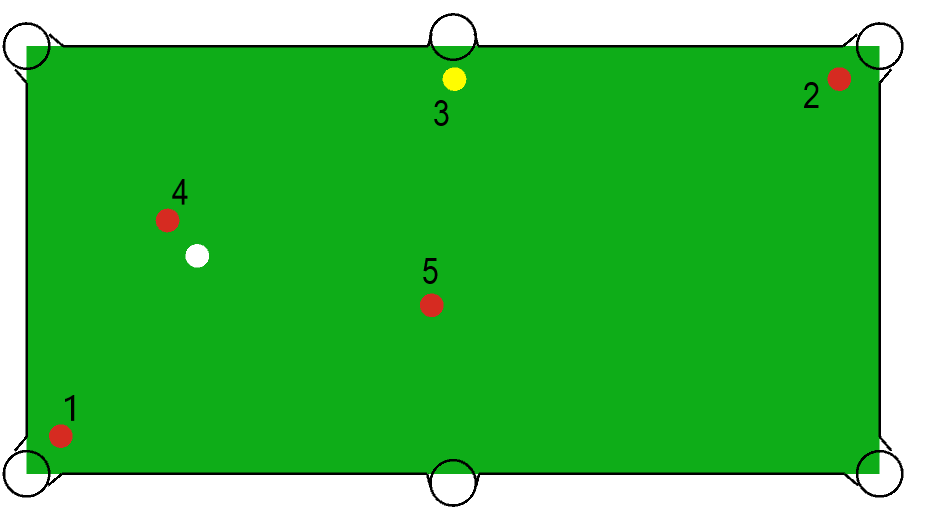
\includegraphics[width=0.4\linewidth]{../common/04_results/resources/simple_search/situation_diverse_deep_search.PNG}
    \end{center}
    \caption{Situation 2: Einige verstreute Kugeln mit einer Gelben}
    \label{fig:search_situation_2}
\end{figure}

In Abbildung \ref{fig:situation_2_solutions} sind die Resultate in aufsteigender Schwierigkeit gegeben. Es wird
jeweils in der linken Spalte der erste Stoss und in der Rechten der darauf basierende zweite Stoss angegeben.

\begin{figure}[h!]
    \centering
    \begin{subfigure}[b]{0.4\textwidth}
        \centering
        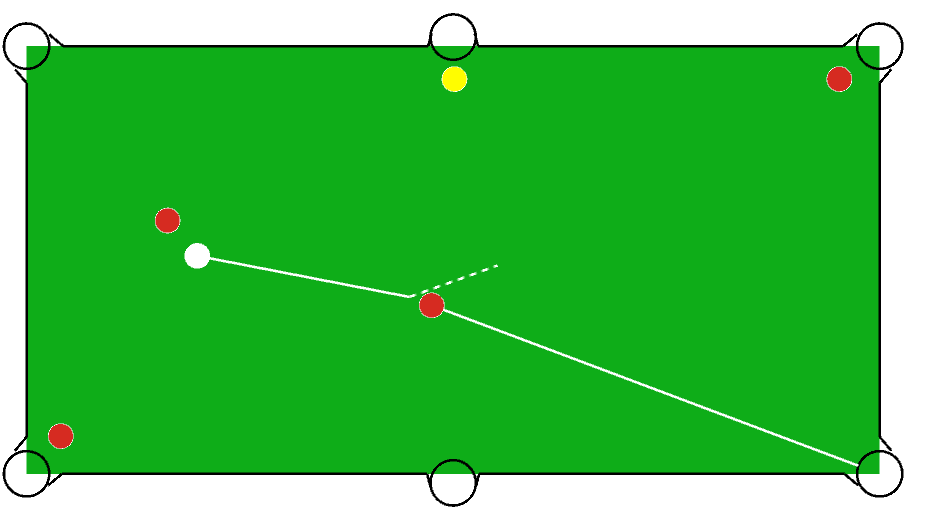
\includegraphics[width=1.0\linewidth]{../common/04_results/resources/simple_search/situation_diverse_solution_deep_search_1a.PNG}
        \caption{Stoss 1-A}
        \label{fig:situation_2_solution_1a}
    \end{subfigure}
    \hfill
    \begin{subfigure}[b]{0.4\textwidth}
        \centering
        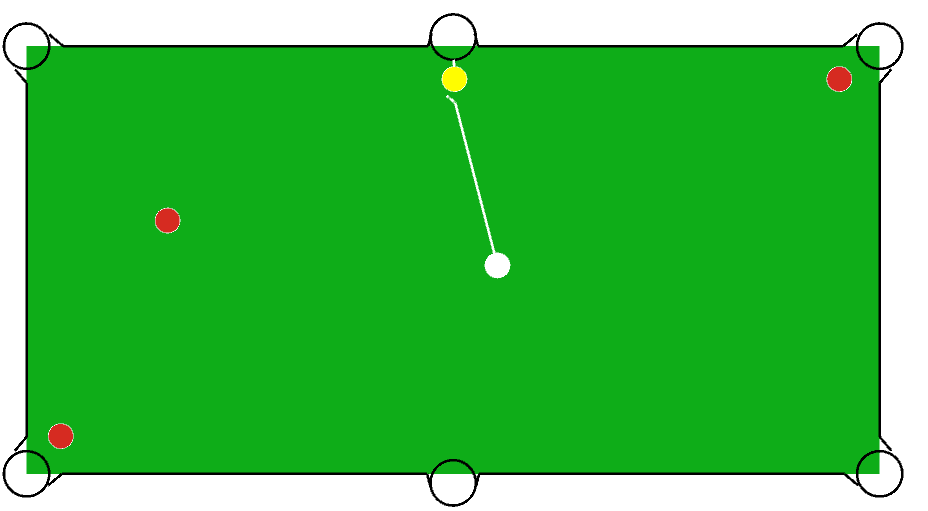
\includegraphics[width=1.0\linewidth]{../common/04_results/resources/simple_search/situation_diverse_solution_deep_search_1b.PNG}
        \caption{Stoss 1-B}
        \label{fig:situation_2_solution_1b}
    \end{subfigure}
    \hfill
    \begin{subfigure}[b]{0.4\textwidth}
        \centering
        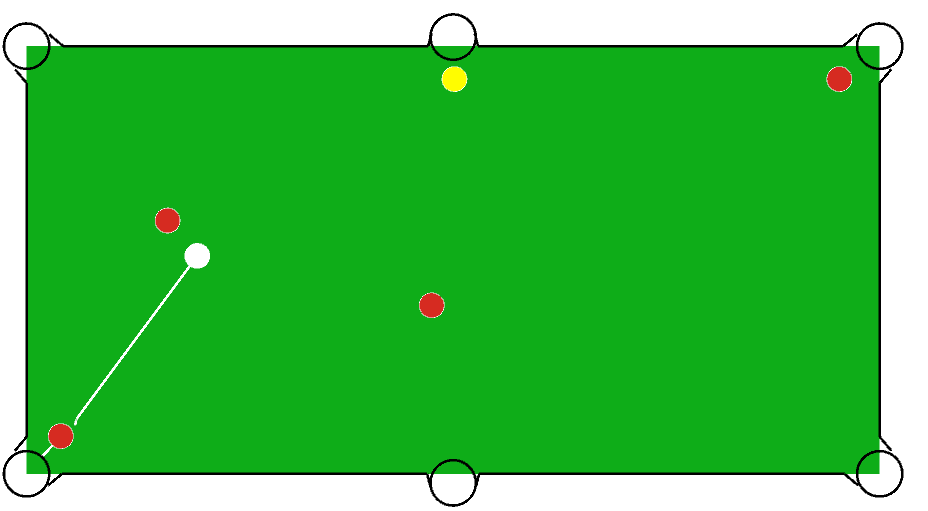
\includegraphics[width=1.0\linewidth]{../common/04_results/resources/simple_search/situation_diverse_solution_deep_search_2a.PNG}
        \caption{Stoss 2-A}
        \label{fig:situation_2_solution_2a}
    \end{subfigure}
    \hfill
    \begin{subfigure}[b]{0.4\textwidth}
        \centering
        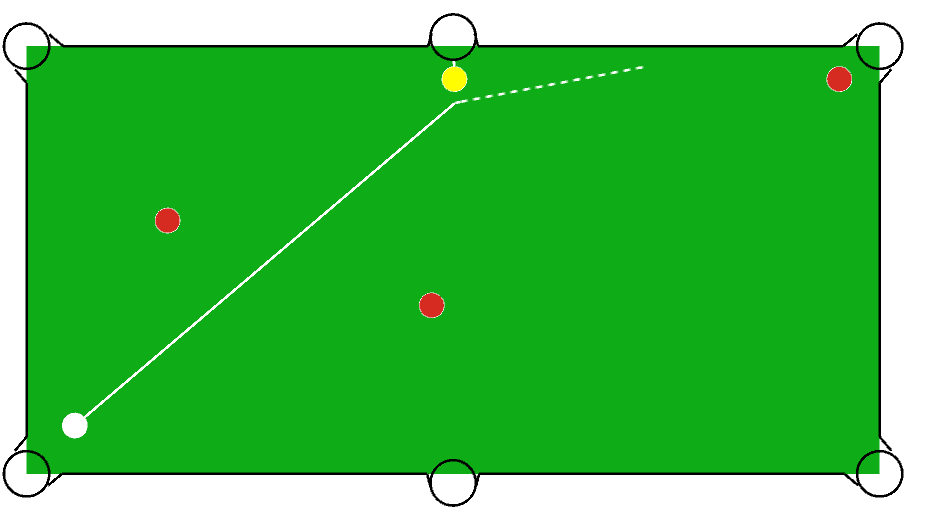
\includegraphics[width=1.0\linewidth]{../common/04_results/resources/simple_search/situation_diverse_solution_deep_search_2b.PNG}
        \caption{Stoss 2-B}
        \label{fig:situation_2_solution_2b}
    \end{subfigure}
    \hfill
    \begin{subfigure}[b]{0.4\textwidth}
        \centering
        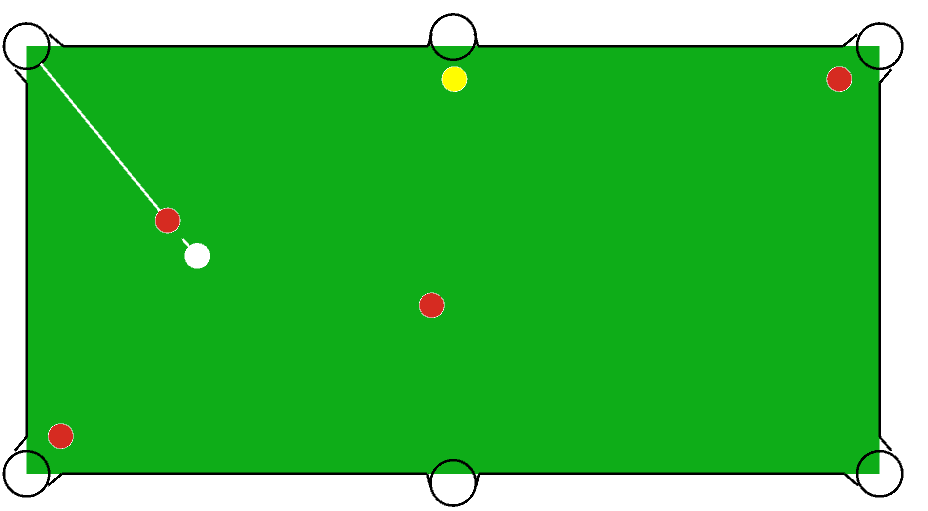
\includegraphics[width=1.0\linewidth]{../common/04_results/resources/simple_search/situation_diverse_solution_deep_search_3a.PNG}
        \caption{Stoss 3-A}
        \label{fig:situation_2_solution_3a}
    \end{subfigure}
    \hfill
    \begin{subfigure}[b]{0.4\textwidth}
        \centering
        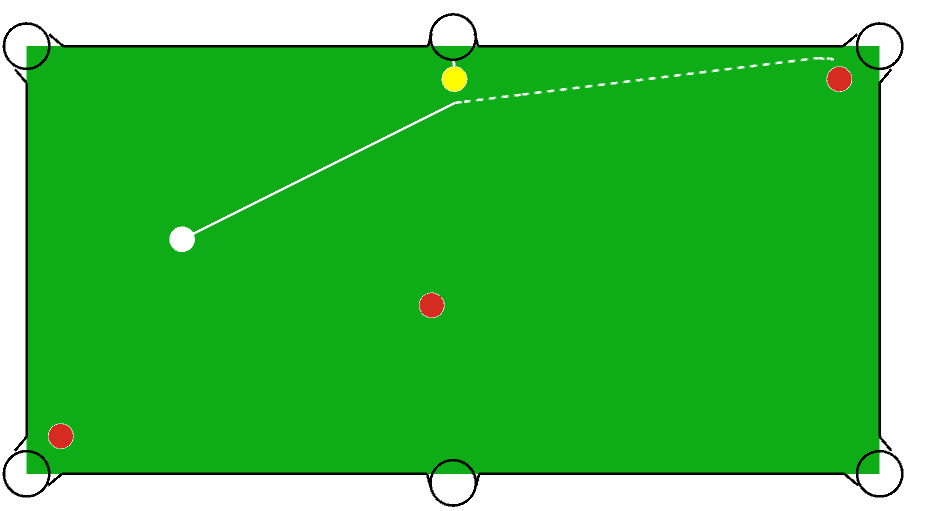
\includegraphics[width=1.0\linewidth]{../common/04_results/resources/simple_search/situation_diverse_solution_deep_search_3b.PNG}
        \caption{Stoss 3-B}
        \label{fig:situation_2_solution_3b}
    \end{subfigure}
    \hfill
    \begin{subfigure}[b]{0.4\textwidth}
        \centering
        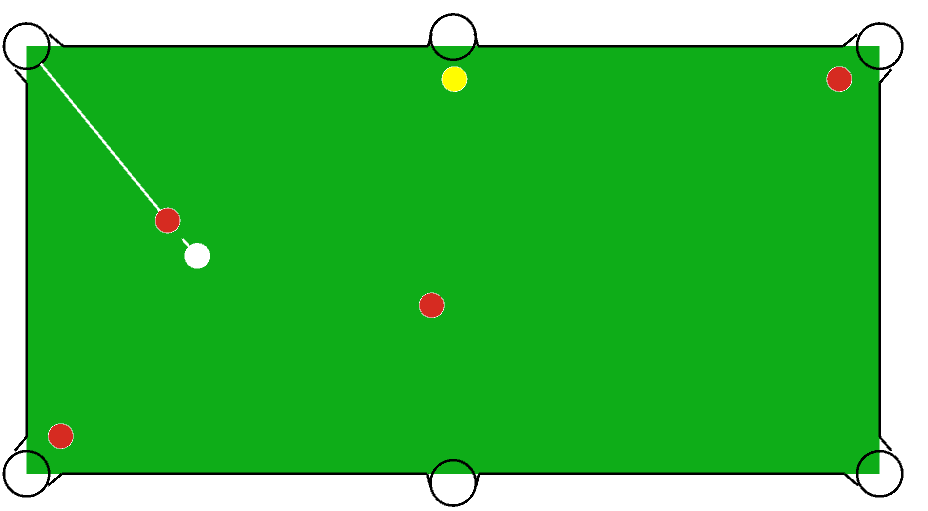
\includegraphics[width=1.0\linewidth]{../common/04_results/resources/simple_search/situation_diverse_solution_deep_search_4a.PNG}
        \caption{Stoss 4-A}
        \label{fig:situation_2_solution_4a}
    \end{subfigure}
    \hfill
    \begin{subfigure}[b]{0.4\textwidth}
        \centering
        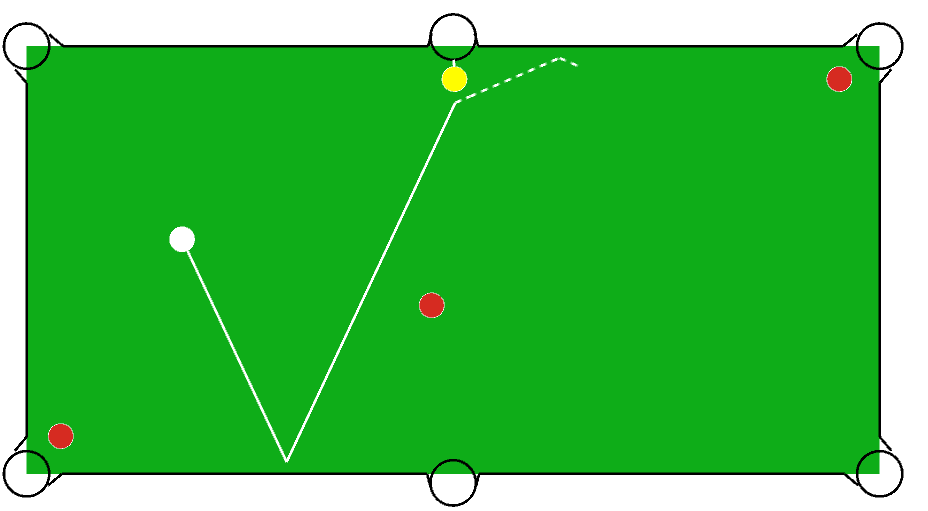
\includegraphics[width=1.0\linewidth]{../common/04_results/resources/simple_search/situation_diverse_solution_deep_search_4b.PNG}
        \caption{Stoss 4-B}
        \label{fig:situation_2_solution_4b}
    \end{subfigure}
    \hfill
    \begin{subfigure}[b]{0.4\textwidth}
        \centering
        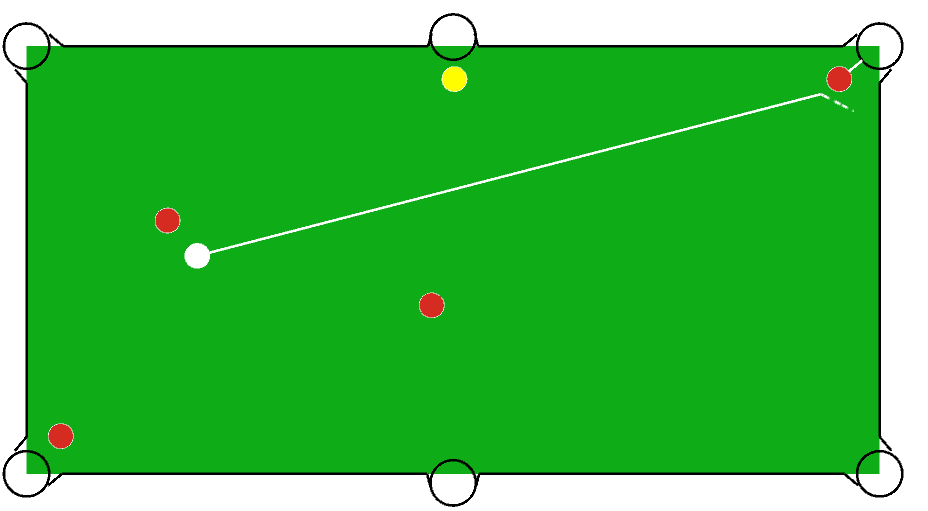
\includegraphics[width=1.0\linewidth]{../common/04_results/resources/simple_search/situation_diverse_solution_deep_search_5a.PNG}
        \caption{Stoss 5-A}
        \label{fig:situation_2_solution_5a}
    \end{subfigure}
    \hfill
    \begin{subfigure}[b]{0.4\textwidth}
        \centering
        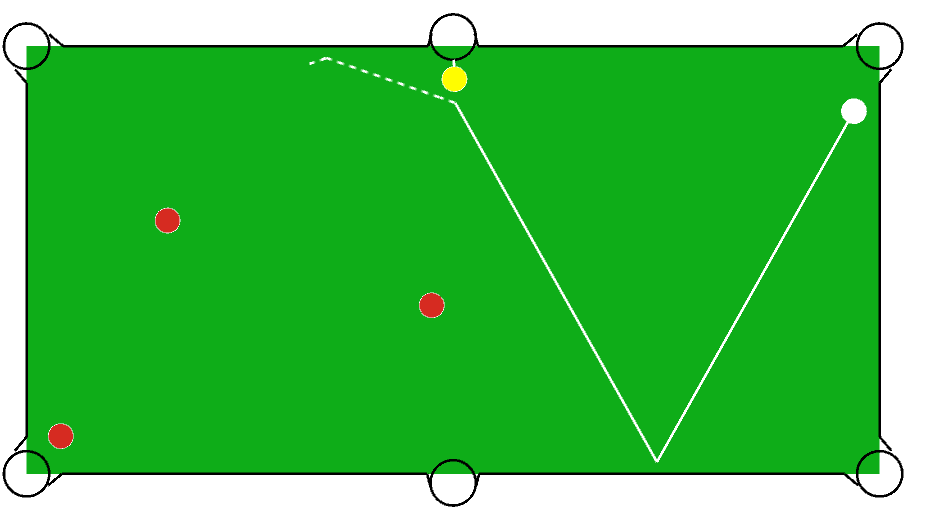
\includegraphics[width=1.0\linewidth]{../common/04_results/resources/simple_search/situation_diverse_solution_deep_search_5b.PNG}
        \caption{Stoss 5-B}
        \label{fig:situation_2_solution_5b}
    \end{subfigure}
    \caption{Gefundene Stösse zu Situation 2 nach bewerteter Schwierigkeit aufsteigend mit darauffolgendem Stoss}
    \label{fig:situation_2_solutions}
\end{figure}

Im Gegensatz zu den vorhergehenden Situationen ist in diesem Fall nicht mehr der Stoss mit der Kugel 1
die beste Wahl. Es wird der zu Beginn etwas komplexere Stoss, welcher die Kugel 5 ins Loch unten
rechts versenkt, vorgeschlagen. Dieser bietet eine optimale Ausgangslage für den darauffolgenden Stoss,
wo die Kugel 3 ins mittlere obere Loch versenkt wird.

Der nächstbeste Stoss ist die Kugel 1 ins untere linke Loch zu versenken und
daraufhin direkt auf die Kugel 3 zu spielen, um sie ebenso wie beim Stoss 1-B im mittleren oberen Loch zu versenken.

In den Stössen 3-A und 4-A wird derselbe Stoss vorgeschlagen, die Kugel 4 im linken oberen Loch zu versenken.
Lediglich die darauf basierenden Stösse 3-B und 4-B unterscheiden sich.
Stoss 3-B spielt die Kugel 3 direkt ins mittlere obere Loch, während Stoss 4-B die Kugel über die untere Bande in dasselbe Loch spielt.
Damit ist Stoss 4-B schwieriger, weil dieser eine Bandeninteraktion enthält und die Distanz grösser ist.

Abschliessend wird das Versenken der Kugel 2 im oberen rechten Loch vorgeschlagen.
Der Stoss 5-B wird über die untere Bande anstelle eines Direkttreffers bevorzugt.
Ein direkter Stoss auf die Kugel 3 würde einen Winkel von praktisch \ang{90} erfordern, was unmöglich wäre.

Mit diesem Kapitel wurden die Vorschläge der Suche von Stössen exemplarisch anhand eines Spielstands erläutert und bewertet.
Eine komplette Analyse weiterer Spielstände unter Berücksichtigung aller Funktionalitäten,
insbesondere der Suche über mehr als zwei Stösse, würde den Rahmen dieses Dokuments sprengen.

Die detaillierte Aufführung der Kosten der Vorschläge sind in den Tabellen \ref{tab:kosten_vorschlag_mehrere_stösse_1},
\ref{tab:kosten_vorschlag_mehrere_stösse_2}, \ref{tab:kosten_vorschlag_mehrere_stösse_3},
\ref{tab:kosten_vorschlag_mehrere_stösse_4} und \ref{tab:kosten_vorschlag_mehrere_stösse_5} aufgeführt.

%%[mapToSolution] COST START
%%[mapToSolution] cost-search - distance: 0 angle: 0 indirection: 0 sum: 0 cost: 0 previous cost: 0 total cost: 0
%%[mapToSolution] cost-search - distance: 0.251514 angle: 0.0224747 indirection: 0 sum: 0.273988 cost: 27398 previous cost: 0 total cost: 27398
%%[mapToSolution] cost-search - distance: 0.0129086 angle: 0.000592332 indirection: 0.5 sum: 0.513501 cost: 51350 previous cost: 27398 total cost: 78748
%%[mapToSolution] cost-simulation - cost: 35872 previous cost: 78748 total cost: 114620
%%[mapToSolution] cost-search - distance: 0 angle: 0 indirection: 0 sum: 0 cost: 0 previous cost: 114620 total cost: 114620
%%[mapToSolution] cost-search - distance: 0.00194371 angle: 7.48391e-07 indirection: 0 sum: 0.00194446 cost: 194 previous cost: 114620 total cost: 114814
%%[mapToSolution] cost-search - distance: 6.02691e-05 angle: 0.0017996 indirection: 0.5 sum: 0.50186 cost: 50185 previous cost: 114814 total cost: 164999
%%[mapToSolution] cost-simulation - cost: 18282 previous cost: 164999 total cost: 183281
%%[mapToSolution] end cost: 183281
%%[mapToSolution] COST END

\begin{table}[h!]
    \rowcolors{1}{\seccolor!10}{\seccolor!10} % Rows with 10% of secondary color
    \begin{tabular}{llrrrr}
        \rowcolor{\seccolor!50}
        Stoss & Segment  & Distanzkosten & Winkelkosten & Indirektionskosten & Total (Ganzzahl)\\\bfhmidline
        1-A          & Weiss - Rot  & 0.0129086     & 0.000592332      & 0.5 & 51350 \\
        1-A          & Rot - Loch   & 0.251514      & 0.0224747        & 0   & 27398 \\
        \textbf{1-A} & \multicolumn{4}{l}{\textbf{Suchkostentotal}}          & \textbf{78748}\\
        1-A          & Simulation   & \multicolumn{4}{r}{35872}\\
        \textbf{1-A} & \multicolumn{4}{l}{\textbf{Zwischentotal}}            & \textbf{114620}\\\bfhmidline
        1-B          & Weiss - Gelb & 0.00006027    & 0.0017996        & 0.5 & 50185 \\
        1-B          & Gelb - Loch  & 0.00194371    & 0.000000748      & 0   & 194 \\
        \textbf{1-B} & \multicolumn{4}{l}{\textbf{Suchkostentotal}}          & \textbf{50379}\\
        1-B          & Simulation & \multicolumn{4}{r}{18282}\\
        \textbf{1-B} & \multicolumn{4}{l}{\textbf{Zwischentotal}}            & \textbf{68661}\\\bfhmidline
        \multicolumn{5}{l}{\textbf{Gesamttotal}}                             & \textbf{183281}\\
    \end{tabular}
    \caption{Detaillierte Kosten von den Stössen 1-A und 1-B aus Abbildung \ref{fig:situation_2_solutions}.}
    \label{tab:kosten_vorschlag_mehrere_stösse_1}
\end{table}

%%[mapToSolution] COST START
%%[mapToSolution] cost-search - distance: 0 angle: 0 indirection: 0 sum: 0 cost: 0 previous cost: 0 total cost: 0
%%[mapToSolution] cost-search - distance: 0.00284364 angle: 3.93338e-06 indirection: 0 sum: 0.00284757 cost: 284 previous cost: 0 total cost: 284
%%[mapToSolution] cost-search - distance: 0.000128041 angle: 7.48246e-05 indirection: 0.5 sum: 0.500203 cost: 50020 previous cost: 284 total cost: 50304
%%[mapToSolution] cost-simulation - cost: 21902 previous cost: 50304 total cost: 72206
%%[mapToSolution] cost-search - distance: 0 angle: 0 indirection: 0 sum: 0 cost: 0 previous cost: 72206 total cost: 72206
%%[mapToSolution] cost-search - distance: 0.00194371 angle: 7.48391e-07 indirection: 0 sum: 0.00194446 cost: 194 previous cost: 72206 total cost: 72400
%%[mapToSolution] cost-search - distance: 0.000531157 angle: 0.319884 indirection: 0.5 sum: 0.820415 cost: 82041 previous cost: 72400 total cost: 154441
%%[mapToSolution] cost-simulation - cost: 30688 previous cost: 154441 [railCombinations] append rail: Right
%%[mapToSolution] end cost: 185129
%%[mapToSolution] COST END

\begin{table}[h!]
    \rowcolors{1}{\seccolor!10}{\seccolor!10} % Rows with 10% of secondary color
    \begin{tabular}{llrrrr}
        \rowcolor{\seccolor!50}
        Stoss & Segment  & Distanzkosten & Winkelkosten & Indirektionskosten & Total (Ganzzahl)\\\bfhmidline
        2-A          & Weiss - Rot  & 0.00012804      & 0.0000748246         & 0.5 & 50020 \\
        2-A          & Rot - Loch   & 0.00284364      & 0.0000039334         & 0   & 284 \\
        \textbf{2-A} & \multicolumn{4}{l}{\textbf{Suchkostentotal}}          & \textbf{50304}\\
        2-A          & Simulation   & \multicolumn{4}{r}{21902}\\
        \textbf{2-A} & \multicolumn{4}{l}{\textbf{Zwischentotal}}            & \textbf{72206}\\\bfhmidline
        2-B          & Weiss - Gelb & 0.000531157    & 0.319884              & 0.5 & 82041 \\
        2-B          & Gelb - Loch  & 0.00194371     & 0.000000748         & 0   & 194 \\
        \textbf{2-B} & \multicolumn{4}{l}{\textbf{Suchkostentotal}}          & \textbf{82235}\\
        2-B          & Simulation & \multicolumn{4}{r}{30688}\\
        \textbf{2-B} & \multicolumn{4}{l}{\textbf{Zwischentotal}}            & \textbf{112923}\\\bfhmidline
        \multicolumn{5}{l}{\textbf{Gesamttotal}}                             & \textbf{185129}\\
    \end{tabular}
    \caption{Detaillierte Kosten von den Stössen 2-A und 2-B aus Abbildung \ref{fig:situation_2_solutions}.}
    \label{tab:kosten_vorschlag_mehrere_stösse_2}
\end{table}

%%[mapToSolution] COST START
%%[mapToSolution] cost-search - distance: 0 angle: 0 indirection: 0 sum: 0 cost: 0 previous cost: 0 total cost: 0
%%[mapToSolution] cost-search - distance: 0.0552051 angle: 9.28795e-05 indirection: 0 sum: 0.055298 cost: 5529 previous cost: 0 total cost: 5529
%%[mapToSolution] cost-search - distance: 3.0656e-05 angle: 2.01923e-06 indirection: 0.5 sum: 0.500033 cost: 50003 previous cost: 5529 total cost: 55532
%%[mapToSolution] cost-simulation - cost: 24388 previous cost: 55532 total cost: 79920
%%[mapToSolution] cost-search - distance: 0 angle: 0 indirection: 0 sum: 0 cost: 0 previous cost: 79920 total cost: 79920
%%[mapToSolution] cost-search - distance: 0.00194371 angle: 7.48391e-07 indirection: 0 sum: 0.00194446 cost: 194 previous cost: 79920 total cost: 80114
%%[mapToSolution] cost-search - distance: 0.000198974 angle: 0.621333 indirection: 0.5 sum: 1.12153 cost: 112153 previous cost: 80114 total cost: 192267
%%[mapToSolution] cost-simulation - cost: 42108 previous cost: 192267 [expandSearchNodeByBank] calculated all combinations: 0
%%[mapToSolution] end cost: 234375
%%[mapToSolution] COST END

\begin{table}[h!]
    \rowcolors{1}{\seccolor!10}{\seccolor!10} % Rows with 10% of secondary color
    \begin{tabular}{llrrrr}
        \rowcolor{\seccolor!50}
        Stoss & Segment  & Distanzkosten & Winkelkosten & Indirektionskosten & Total (Ganzzahl)\\\bfhmidline
        3-A          & Weiss - Rot  & 0.00003066     & 0.0000020193          & 0.5 & 50003 \\
        3-A          & Rot - Loch   & 0.0552051      & 0.0000928795          & 0   & 5529 \\
        \textbf{3-A} & \multicolumn{4}{l}{\textbf{Suchkostentotal}}          & \textbf{55532}\\
        3-A          & Simulation   & \multicolumn{4}{r}{24388}\\
        \textbf{3-A} & \multicolumn{4}{l}{\textbf{Zwischentotal}}            & \textbf{79920}\\\bfhmidline
        3-B          & Weiss - Gelb & 0.000198974    & 0.621333              & 0.5 & 112153 \\
        3-B          & Gelb - Loch  & 0.00194371     & 0.000000748           & 0   & 194 \\
        \textbf{3-B} & \multicolumn{4}{l}{\textbf{Suchkostentotal}}          & \textbf{112347}\\
        3-B          & Simulation & \multicolumn{4}{r}{42108}\\
        \textbf{3-B} & \multicolumn{4}{l}{\textbf{Zwischentotal}}            & \textbf{154455}\\\bfhmidline
        \multicolumn{5}{l}{\textbf{Gesamttotal}}                             & \textbf{234375}\\
    \end{tabular}
    \caption{Detaillierte Kosten von den Stössen 3-A und 3-B aus Abbildung \ref{fig:situation_2_solutions}.}
    \label{tab:kosten_vorschlag_mehrere_stösse_3}
\end{table}

%%[mapToSolution] COST START
%%[mapToSolution] cost-search - distance: 0 angle: 0 indirection: 0 sum: 0 cost: 0 previous cost: 0 total cost: 0
%%[mapToSolution] cost-search - distance: 0.0552051 angle: 9.28795e-05 indirection: 0 sum: 0.055298 cost: 5529 previous cost: 0 total cost: 5529
%%[mapToSolution] cost-search - distance: 3.0656e-05 angle: 2.01923e-06 indirection: 0.5 sum: 0.500033 cost: 50003 previous cost: 5529 total cost: 55532
%%[mapToSolution] cost-simulation - cost: 24388 previous cost: 55532 total cost: 79920
%%[mapToSolution] cost-search - distance: 0 angle: 0 indirection: 0 sum: 0 cost: 0 previous cost: 79920 total cost: 79920
%%[mapToSolution] cost-search - distance: 0.00194371 angle: 7.48391e-07 indirection: 0 sum: 0.00194446 cost: 194 previous cost: 79920 total cost: 80114
%%[mapToSolution] cost-search - distance: 0.000465118 angle: 0.0581145 indirection: 1.16667 sum: 1.22525 cost: 122524 previous cost: 80114 total cost: 202638
%%[mapToSolution] cost-simulation - cost: 51021 previous cost: 202638 [railTargets] calculate next target with reflected point (-2707.76, 443.306) from start(93.1251, 422.377) at rail Left
%%[mapToSolution] end cost: 253659
%%[mapToSolution] COST END

\begin{table}[h!]
    \rowcolors{1}{\seccolor!10}{\seccolor!10} % Rows with 10% of secondary color
    \begin{tabular}{llrrrr}
        \rowcolor{\seccolor!50}
        Stoss & Segment  & Distanzkosten & Winkelkosten & Indirektionskosten & Total (Ganzzahl)\\\bfhmidline
        4-A          & Weiss - Rot  & 0.00003066     & 0.0000020193          & 0.5 & 50003 \\
        4-A          & Rot - Loch   & 0.0552051      & 0.0000928795          & 0   & 5529 \\
        \textbf{4-A} & \multicolumn{4}{l}{\textbf{Suchkostentotal}}          & \textbf{55532}\\
        4-A          & Simulation   & \multicolumn{4}{r}{24388}\\
        \textbf{4-A} & \multicolumn{4}{l}{\textbf{Zwischentotal}}            & \textbf{79920}\\\bfhmidline
        4-B          & Weiss - Gelb & 0.000465118    & 0.0581145             & 1.167 & 122524 \\
        4-B          & Gelb - Loch  & 0.00194371     & 0.000000748           & 0   & 194 \\
        \textbf{4-B} & \multicolumn{4}{l}{\textbf{Suchkostentotal}}          & \textbf{122718}\\
        4-B          & Simulation & \multicolumn{4}{r}{51021}\\
        \textbf{4-B} & \multicolumn{4}{l}{\textbf{Zwischentotal}}            & \textbf{173739}\\\bfhmidline
        \multicolumn{5}{l}{\textbf{Gesamttotal}}                             & \textbf{253659}\\
    \end{tabular}
    \caption{Detaillierte Kosten von den Stössen 4-A und 4-B aus Abbildung \ref{fig:situation_2_solutions}.}
    \label{tab:kosten_vorschlag_mehrere_stösse_4}
\end{table}

%%[mapToSolution] COST START
%%[mapToSolution] cost-search - distance: 0 angle: 0 indirection: 0 sum: 0 cost: 0 previous cost: 0 total cost: 0
%%[mapToSolution] cost-search - distance: 0.0029786 angle: 7.36014e-05 indirection: 0 sum: 0.0030522 cost: 305 previous cost: 0 total cost: 305
%%[mapToSolution] cost-search - distance: 0.00135804 angle: 0.0237772 indirection: 0.5 sum: 0.525135 cost: 52513 previous cost: 305 total cost: 52818
%%[mapToSolution] cost-simulation - cost: 23547 previous cost: 52818 total cost: 76365
%%[mapToSolution] cost-search - distance: 0 angle: 0 indirection: 0 sum: 0 cost: 0 previous cost: 76365 total cost: 76365
%%[mapToSolution] cost-search - distance: 0.00194371 angle: 7.48391e-07 indirection: 0 sum: 0.00194446 cost: 194 previous cost: 76365 total cost: 76559
%%[mapToSolution] cost-search - distance: 0.000707568 angle: 0.0805186 indirection: 1.16667 sum: 1.24789 cost: 124789 previous cost: 76559 total cost: 201348
%%[mapToSolution] cost-simulation - cost: 52613 previous cost: 201348 total cost: 253961
%%[mapToSolution] end cost: 253961
%%[mapToSolution] COST END

\begin{table}[h!]
    \rowcolors{1}{\seccolor!10}{\seccolor!10} % Rows with 10% of secondary color
    \begin{tabular}{llrrrr}
        \rowcolor{\seccolor!50}
        Stoss & Segment  & Distanzkosten & Winkelkosten & Indirektionskosten & Total (Ganzzahl)\\\bfhmidline
        5-A          & Rot - Loch   & 0.0029786      & 0.0000736014          & 0   & 305 \\
        5-A          & Weiss - Rot  & 0.00135804      & 0.0237772            & 0.5 & 52513 \\
        \textbf{5-A} & \multicolumn{4}{l}{\textbf{Suchkostentotal}}          & \textbf{52818}\\
        5-A          & Simulation   & \multicolumn{4}{r}{23547}\\
        \textbf{5-A} & \multicolumn{4}{l}{\textbf{Zwischentotal}}            & \textbf{76365}\\\bfhmidline
        5-B          & Weiss - Gelb & 0.000707568    & 0.0805186             & 1.167 & 124789 \\
        5-B          & Gelb - Loch  & 0.00194371     & 0.000000748           & 0   & 194 \\
        \textbf{5-B} & \multicolumn{4}{l}{\textbf{Suchkostentotal}}          & \textbf{124983}\\
        5-B          & Simulation & \multicolumn{4}{r}{52613}\\
        \textbf{5-B} & \multicolumn{4}{l}{\textbf{Zwischentotal}}            & \textbf{177596}\\\bfhmidline
        \multicolumn{5}{l}{\textbf{Gesamttotal}}                             & \textbf{253961}\\
    \end{tabular}
    \caption{Detaillierte Kosten von den Stössen 5-A und 5-B aus Abbildung \ref{fig:situation_2_solutions}.}
    \label{tab:kosten_vorschlag_mehrere_stösse_5}
\end{table}
